\chapter{Experiments and Results}
\label{chap:experiments_results}

This chapter delineates the experimental methodologies and presents the findings from a series of evaluations conducted to assess various components and strategies within Retrieval-Augmented Generation systems. The experiments encompass a spectrum of techniques, ranging from fundamental retrieval and chunking methods to advanced reranking, prompt engineering, and the influence of different embedding and generative models. The overarching objective is to identify optimal configurations for robust and effective RAG pipelines.

\section{General Experimental Setup}
\label{sec:general_setup}
To ensure a systematic and reproducible evaluation, all experiments were conducted employing a consistent setup.

\subsection{Dataset(s)}
The primary dataset utilized for these experiments comprises a curated collection of academic papers and articles pertaining to the field of artificial intelligence. This dataset was selected due to its inherent complexity, specialized technical vocabulary, and the requirement for precise, fact-based answers. For question generation and evaluation, a set of 100 questions was meticulously crafted, encompassing a range of topics within the dataset. Each question is formulated to possess a verifiable answer within the document corpus.

\subsection{Baseline Configuration}
To quantify the impact of various optimization techniques, a baseline RAG configuration was established:
\begin{itemize}
    \item \textbf{Embedding Model:} OpenAI \texttt{text-embedding-ada-002}, a widely adopted and robust baseline model.
    \item \textbf{Chunking Strategy:} Naive fixed-size chunking, employing a chunk size of 300 tokens and an overlap of 50 tokens.
    \item \textbf{Retrieval Strategy:} Basic cosine similarity search, with a predetermined retrieval of the top 5 most similar chunks (Top-N).
    \item \textbf{Generator LLM:} \texttt{GPT-4}.
    \item \textbf{Prompt Template:} A standard zero-shot prompt directing the LLM to formulate its answer based on the provided context.
\end{itemize}

\subsection{Core Evaluation Metrics}
The performance of the RAG system was assessed at both the retrieval and generation stages.
\begin{itemize}
\item \textbf{Retrieval Performance:} Evaluated using \textit{Precision@k}, \textit{Recall@k}, and \textit{Mean Reciprocal Rank (MRR)}. These metrics are paramount for comprehending the effectiveness of the retrieval stage in isolation.
\item \textbf{Generation Quality:} Assessed using the \textit{LLM-as-a-Judge} method with the DeepEval framework. The primary metrics tracked were \textit{Faithfulness}, \textit{Answer Relevancy}, and \textit{Hallucination Rate} \autocite{zheng2023judging}.
\end{itemize}

\section{Experiment 1: Embedding Models}
\label{sec:exp_embedding_models}
This experiment assesses the performance of various embedding models on long-context retrieval tasks. The objective is to comprehend how diverse architectural and chunking strategies influence retrieval performance on documents of varying lengths and complexity.

\subsection{Models and Methodology}
We compared five embedding models on the \textbf{LongEmbed} benchmark \autocite{zhu2024longembedextendingembeddingmodels}, a suite of datasets formulated to evaluate long-context retrieval. The models assessed were:
\begin{itemize}
    \item \textbf{OpenAI \texttt{text-embedding-ada-002}:} A widely adopted, high-performance proprietary model with a vector size of 1536. This model does not necessitate any specific task instruction.
    \item \textbf{Nomic AI \texttt{nomic-embed-text}:} An open-source model possessing a vector size of 768. This model employs a prefix for distinct tasks. For our retrieval task, we used `search\_query:` for queries and `search\_document:` for documents.
    \item \textbf{Jina AI \texttt{jina-embeddings-v2-base-en}:} An open-source model with a vector size of 768. This model, like Ada-002, does not require a task instruction.
    \item \textbf{Jina AI \texttt{jina-embeddings-v3}:} A model that implements \textit{late chunking}, where chunks from the same document are tokenized together up to the model's context window of 8192 tokens, with a vector size of 1024. It requires a `task` argument, for which we used `retrieval.query` and `retrieval.passage` for queries and documents respectively.
    \item \textbf{Qwen \texttt{Qwen3-Embedding-0.6B}:} An open-source model with a vector size of 1024. This model benefits from a prompt for queries, for which we used the recommended `query` prompt name.
\end{itemize}
For vector storage and retrieval, we used Milvus \autocite{milvus}, a popular open-source vector database. We created an index of type HNSW (Hierarchical Navigable Small World) with the L2 distance metric. The index parameters were set to M=8 and efConstruction=64.

\subsection{Datasets}
The LongEmbed benchmark comprises six datasets, two of which are synthetic and four are derived from real-world data. The datasets are:
\begin{itemize}
    \item \textbf{2WikiMQA:} A multi-hop question-answering dataset.
    \item \textbf{NarrativeQA:} A question-answering dataset featuring extended narratives.
    \item \textbf{Needle In A Haystack (NIAH):} A synthetic dataset designed to evaluate the model's capacity to locate a specific piece of information ("needle") in an extensive text ("haystack").
    \item \textbf{Passkey Retrieval:} A synthetic dataset designed to assess the model's ability to retrieve a specific key from an extended document.
    \item \textbf{QMSum:} A query-based meeting summarization dataset.
    \item \textbf{SummScreenFD:} A summarization dataset derived from television show scripts.
\end{itemize}

\subsection{Results and Discussion}
The retrieval performance of the five embedding models across the six datasets is presented in detail in Tables~\ref{tab:detailed_recall} through~\ref{tab:detailed_nDCG}, with an aggregated summary provided in Table~\ref{tab:summary}. The results not only underscore a clear superior performer within our long-context benchmark but also indicate a significant paradigm shift in the broader landscape of text embedding models.

\paragraph{The Rise of Compact, High-Performance Models}
While our results identify \textbf{\texttt{Qwen3-Embedding-0.6B}} as the leading performer, its true significance becomes apparent when contextualized within the global Massive Text Embedding Benchmark (MTEB) leaderboard. As of August 1st, 2025, this model occupies an impressive 4th rank overall, surpassed solely by Google's proprietary \texttt{gemini-embedding-001} and its own, substantially larger 4B and 8B parameter siblings \autocite{mteb_leaderboard_2025}. With merely 595M parameters, its performance is noteworthy, demonstrating that architectural innovations and advanced training pipelines can enable smaller, open-source models to surpass the performance of significantly larger competitors. This efficiency stems directly from its foundation on the Qwen3 architecture \autocite{yang2025qwen3technicalreport} and a sophisticated multi-stage training process that leverages the foundational LLM itself to synthesize high-quality training data \autocite{zhang2025qwen3embeddingadvancingtext}.

\paragraph{A New Baseline: The Obsolescence of Ada-002}
For years, OpenAI's \textbf{\texttt{ada-002}} served as a de facto industry standard. However, these results, coupled with its MTEB ranking of 167th, confirm that it has been decisively superseded. Newer models, leveraging innovative architectures and specialized training techniques, now provide substantially superior performance. The other models in our evaluation also rank significantly higher than \texttt{ada-002} on the MTEB leaderboard: \texttt{jina-embeddings-v3} ranks 24th, \texttt{nomic-embed-text} ranks 54th, and even the earlier \texttt{jina-embeddings-v2-base-en} ranks 154th \autocite{mteb_leaderboard_2025}. This trend indicates that the benchmark for state-of-the-art has shifted towards more open and efficient models.

\paragraph{The Enduring Value of Specialization}
Despite the prevalence of a robust generalist model like Qwen3, our findings also emphasize the persistent importance of specialized models. \textbf{\texttt{jina-embeddings-v3}}, with its unique late chunking strategy, maintains its position as the leading performer on the \texttt{passkey} task, thereby validating the efficacy of its architectural design for retrieving specific facts from structured long documents. Similarly, \textbf{\texttt{nomic-embed-text}}'s superior performance on the \texttt{needle} dataset affirms its designation as a premier model for extreme "needle-in-a-haystack" scenarios. This demonstrates that for specific, challenging use cases, a specialized model can remain the optimal choice.

\paragraph{Distance Metrics and Model Compatibility}
For most models, the selection between L2 and Inner Product (IP) distance metrics yields comparable results, indicating that their embeddings are adequately normalized. A crucial observation, however, pertains to the performance degradation of \textbf{\texttt{jina-embeddings-v2-base-en}} when employing the IP metric. As observed across all tables, its performance significantly diminishes with IP; for instance, its average Recall@5 decreases from 51.85\% (L2) to a mere 12.12\% (IP). This underscores that its embedding vectors are not normalized for cosine similarity, rendering L2 distance the sole viable choice for this model and emphasizing the importance of aligning the retrieval metric with the model's output properties.

\paragraph{Conclusion}
In summary, this experiment exemplifies a pivotal moment in the evolution of text embedding models. Our findings lead to the following conclusions:
\begin{itemize}
    \item The embedding landscape is no longer dominated by large, proprietary models. The exceptional performance of \textbf{\texttt{Qwen3-Embedding-0.6B}}, a compact 595M parameter model, indicates a shift towards more efficient, accessible, and open-source solutions that attain state-of-the-art results.
    \item Models such as \textbf{\texttt{ada-002}}, while historically significant, are now considered obsolete. They have been superseded by a new generation of models featuring more advanced architectures, training methodologies, and specialized strategies such as late chunking.
    \item While general-purpose models have improved substantially, \textbf{specialization remains highly valuable}. For niche but critical tasks such as extreme long-context fact retrieval, models like \texttt{jina-embeddings-v3} and \texttt{nomic-embed-text} offer targeted performance that can surpass even the most proficient generalists.
    \item \textbf{Technical implementation details are paramount}. The selection of the distance metric must be compatible with the model's properties, as the suboptimal performance of \texttt{jina-embeddings-v2-base-en} with the IP metric illustrates.
\end{itemize}

\begin{sidewaystable}[htbp!]
\centering
\footnotesize
\captionof{table}{Detailed RECALL Performance (in \%). Higher is better. Results are grouped by k-value. Best result per column within each k-value group is in \textbf{bold}.}
\label{tab:detailed_recall}
\begin{tabular}{llcccccccccccccc}
\toprule
\multirow{2}{*}{k} & \multirow{2}{*}{Model} & \multicolumn{2}{c}{2wikimqa} & \multicolumn{2}{c}{narrativeqa} & \multicolumn{2}{c}{needle} & \multicolumn{2}{c}{passkey} & \multicolumn{2}{c}{qmsum} & \multicolumn{2}{c}{summ screen fd} & \multicolumn{2}{c}{Average} \\
\cmidrule(lr){3-4} \cmidrule(lr){5-6} \cmidrule(lr){7-8} \cmidrule(lr){9-10} \cmidrule(lr){11-12} \cmidrule(lr){13-14} \cmidrule(lr){15-16}
& & L2 & IP & L2 & IP & L2 & IP & L2 & IP & L2 & IP & L2 & IP & L2 & IP \\
\midrule
\multirow{5}{*}{1} & Ada-002 & 79.33 & 81.00 & 54.44 & 54.27 & 2.00 & 1.50 & \textbf{13.25} & \textbf{14.50} & 45.65 & 45.91 & 86.90 & 86.90 & 52.01 & 51.98 \\
& Jina-V2 & \textbf{91.67} & 24.67 & 41.43 & 2.32 & 3.75 & 0.00 & 12.75 & 8.00 & 40.54 & 11.07 & 81.55 & 32.14 & 41.48 & 4.66 \\
& Jina-V3 & 90.67 & \textbf{90.67} & 57.54 & 57.46 & 1.25 & 0.75 & 10.50 & 12.50 & 47.22 & 47.22 & 84.23 & 84.23 & 54.69 & 54.67 \\
& Nomic & 67.33 & 67.33 & 47.51 & 48.15 & \textbf{8.75} & \textbf{9.25} & 5.75 & 3.75 & 21.02 & 21.02 & 52.98 & 52.98 & 42.67 & 43.13 \\
& Qwen3-0.6B & 89.67 & 89.67 & \textbf{62.99} & \textbf{62.85} & 4.25 & 3.75 & 9.50 & 13.75 & \textbf{50.49} & \textbf{50.49} & \textbf{88.10} & \textbf{88.10} & \textbf{59.45} & \textbf{59.45} \\
\midrule
\multirow{5}{*}{5} & Ada-002 & 87.33 & 88.00 & 63.85 & 63.64 & 4.25 & 4.00 & 32.50 & 34.00 & 65.82 & 66.34 & 96.73 & 96.73 & 62.71 & 62.66 \\
& Jina-V2 & 95.67 & 66.00 & 50.31 & 6.02 & 5.75 & 0.00 & 29.50 & 15.25 & 62.08 & 32.87 & 95.54 & 69.94 & 51.85 & 12.12 \\
& Jina-V3 & \textbf{96.67} & \textbf{96.67} & 67.40 & 67.42 & 2.00 & 2.00 & \textbf{40.50} & \textbf{44.50} & 67.58 & 67.58 & 97.92 & 97.92 & 66.09 & 66.22 \\
& Nomic & 79.67 & 79.67 & 58.64 & 59.33 & \textbf{14.50} & \textbf{14.75} & 9.25 & 5.25 & 39.03 & 39.03 & 82.74 & 82.74 & 54.69 & 55.11 \\
& Qwen3-0.6B & 95.67 & 95.67 & \textbf{73.27} & \textbf{73.16} & 5.50 & 6.50 & 15.75 & 40.75 & \textbf{72.30} & \textbf{72.30} & \textbf{98.21} & \textbf{98.21} & \textbf{70.55} & \textbf{71.23} \\
\midrule
\multirow{5}{*}{10} & Ada-002 & 90.00 & 90.67 & 66.35 & 66.22 & 5.25 & 5.00 & 38.75 & 41.00 & 73.94 & 74.46 & \textbf{98.81} & \textbf{98.81} & 65.91 & 65.94 \\
& Jina-V2 & 97.67 & 77.67 & 53.39 & 7.71 & 6.25 & 0.25 & 31.25 & 16.50 & 72.30 & 45.12 & 97.62 & 81.85 & 55.58 & 15.43 \\
& Jina-V3 & \textbf{98.33} & \textbf{98.33} & 70.67 & 70.71 & 2.25 & 2.50 & \textbf{53.50} & \textbf{58.75} & 75.05 & 75.05 & \textbf{98.81} & \textbf{98.81} & 69.94 & 70.13 \\
& Nomic & 85.00 & 85.00 & 62.32 & 62.88 & \textbf{17.25} & \textbf{17.50} & 9.25 & 5.25 & 47.35 & 47.35 & 91.07 & 91.07 & 58.92 & 59.24 \\
& Qwen3-0.6B & 98.00 & 98.00 & \textbf{76.48} & \textbf{76.18} & 6.25 & 7.00 & 16.00 & 42.25 & \textbf{79.96} & \textbf{79.96} & 98.21 & 98.21 & \textbf{74.00} & \textbf{74.58} \\
\midrule
\multirow{5}{*}{25} & Ada-002 & 92.33 & 92.67 & 69.44 & 69.45 & 7.50 & 7.50 & 49.75 & 53.25 & 82.25 & 82.91 & \textbf{99.70} & \textbf{99.70} & 69.74 & 69.93 \\
& Jina-V2 & 98.67 & 91.67 & 56.97 & 11.65 & 8.50 & 1.50 & 33.25 & 17.75 & 81.99 & 64.37 & 97.92 & 93.45 & 59.63 & 21.37 \\
& Jina-V3 & \textbf{99.33} & \textbf{99.33} & 74.30 & 74.28 & 5.25 & 5.25 & \textbf{54.25} & \textbf{60.00} & 83.76 & 83.76 & \textbf{99.70} & \textbf{99.70} & 73.92 & 74.08 \\
& Nomic & 89.33 & 89.33 & 66.78 & 67.31 & \textbf{20.00} & \textbf{19.75} & 9.25 & 5.25 & 62.41 & 62.41 & 96.13 & 96.13 & 64.41 & 64.70 \\
& Qwen3-0.6B & 98.33 & 98.33 & \textbf{79.88} & \textbf{79.71} & 8.25 & 11.25 & 16.00 & 42.25 & \textbf{89.00} & \textbf{89.00} & \textbf{99.70} & \textbf{99.70} & \textbf{77.79} & \textbf{78.53} \\
\bottomrule
\end{tabular}
\end{sidewaystable}
\clearpage
\begin{sidewaystable}[htbp!]
\centering
\footnotesize
\captionof{table}{Detailed PRECISION Performance (in \%). Higher is better. Results are grouped by k-value. Best result per column within each k-value group is in \textbf{bold}.}
\label{tab:detailed_precision}
\begin{tabular}{llcccccccccccccc}
\toprule
\multirow{2}{*}{k} & \multirow{2}{*}{Model} & \multicolumn{2}{c}{2wikimqa} & \multicolumn{2}{c}{narrativeqa} & \multicolumn{2}{c}{needle} & \multicolumn{2}{c}{passkey} & \multicolumn{2}{c}{qmsum} & \multicolumn{2}{c}{summ screen fd} & \multicolumn{2}{c}{Average} \\
\cmidrule(lr){3-4} \cmidrule(lr){5-6} \cmidrule(lr){7-8} \cmidrule(lr){9-10} \cmidrule(lr){11-12} \cmidrule(lr){13-14} \cmidrule(lr){15-16}
& & L2 & IP & L2 & IP & L2 & IP & L2 & IP & L2 & IP & L2 & IP & L2 & IP \\
\midrule
\multirow{5}{*}{1} & Ada-002 & 79.33 & 81.00 & 54.44 & 54.27 & 2.00 & 1.50 & \textbf{13.25} & \textbf{14.50} & 45.65 & 45.91 & 86.90 & 86.90 & 52.01 & 51.98 \\
& Jina-V2 & \textbf{91.67} & 24.67 & 41.43 & 2.32 & 3.75 & 0.00 & 12.75 & 8.00 & 40.54 & 11.07 & 81.55 & 32.14 & 41.48 & 4.66 \\
& Jina-V3 & 90.67 & \textbf{90.67} & 57.54 & 57.46 & 1.25 & 0.75 & 10.50 & 12.50 & 47.22 & 47.22 & 84.23 & 84.23 & 54.69 & 54.67 \\
& Nomic & 67.33 & 67.33 & 47.51 & 48.15 & \textbf{8.75} & \textbf{9.25} & 5.75 & 3.75 & 21.02 & 21.02 & 52.98 & 52.98 & 42.67 & 43.13 \\
& Qwen3-0.6B & 89.67 & 89.67 & \textbf{62.99} & \textbf{62.85} & 4.25 & 3.75 & 9.50 & 13.75 & \textbf{50.49} & \textbf{50.49} & \textbf{88.10} & \textbf{88.10} & \textbf{59.45} & \textbf{59.45} \\
\midrule
\multirow{5}{*}{5} & Ada-002 & 17.47 & 17.60 & 12.77 & 12.73 & 0.85 & 0.80 & 6.50 & 6.80 & 13.16 & 13.27 & 19.35 & 19.35 & 12.54 & 12.53 \\
& Jina-V2 & 19.13 & 13.20 & 10.06 & 1.20 & 1.15 & 0.00 & 5.90 & 3.05 & 12.42 & 6.57 & 19.11 & 13.99 & 10.37 & 2.42 \\
& Jina-V3 & \textbf{19.33} & \textbf{19.33} & 13.48 & 13.48 & 0.40 & 0.40 & \textbf{8.10} & \textbf{8.90} & 13.52 & 13.52 & 19.58 & 19.58 & 13.22 & 13.24 \\
& Nomic & 15.93 & 15.93 & 11.73 & 11.87 & \textbf{2.90} & \textbf{2.95} & 1.85 & 1.05 & 7.81 & 7.81 & 16.55 & 16.55 & 10.94 & 11.02 \\
& Qwen3-0.6B & 19.13 & 19.13 & \textbf{14.65} & \textbf{14.63} & 1.10 & 1.30 & 3.15 & 8.15 & \textbf{14.46} & \textbf{14.46} & \textbf{19.64} & \textbf{19.64} & \textbf{14.11} & \textbf{14.25} \\
\midrule
\multirow{5}{*}{10} & Ada-002 & 9.00 & 9.07 & 6.64 & 6.62 & 0.53 & 0.50 & 3.87 & 4.10 & 7.39 & 7.45 & \textbf{9.88} & \textbf{9.88} & 6.59 & 6.59 \\
& Jina-V2 & 9.77 & 7.77 & 5.34 & 0.77 & 0.63 & 0.03 & 3.12 & 1.65 & 7.23 & 4.51 & 9.76 & 8.18 & 5.56 & 1.54 \\
& Jina-V3 & \textbf{9.83} & \textbf{9.83} & 7.07 & 7.07 & 0.22 & 0.25 & \textbf{5.35} & \textbf{5.88} & 7.50 & 7.50 & \textbf{9.88} & \textbf{9.88} & 6.99 & 7.01 \\
& Nomic & 8.50 & 8.50 & 6.23 & 6.29 & \textbf{1.72} & \textbf{1.75} & 0.93 & 0.53 & 4.73 & 4.73 & 9.11 & 9.11 & 5.89 & 5.92 \\
& Qwen3-0.6B & 9.80 & 9.80 & \textbf{7.65} & \textbf{7.62} & 0.63 & 0.70 & 1.60 & 4.22 & \textbf{8.00} & \textbf{8.00} & 9.82 & 9.82 & \textbf{7.40} & \textbf{7.46} \\
\midrule
\multirow{5}{*}{25} & Ada-002 & 3.69 & 3.71 & 2.78 & 2.78 & 0.30 & 0.30 & 1.99 & 2.13 & 3.29 & 3.32 & \textbf{3.99} & \textbf{3.99} & 2.79 & 2.80 \\
& Jina-V2 & 3.95 & 3.67 & 2.28 & 0.47 & 0.34 & 0.06 & 1.33 & 0.71 & 3.28 & 2.57 & 3.92 & 3.74 & 2.39 & 0.85 \\
& Jina-V3 & \textbf{3.97} & \textbf{3.97} & 2.97 & 2.97 & 0.21 & 0.21 & \textbf{2.17} & \textbf{2.40} & 3.35 & 3.35 & \textbf{3.99} & \textbf{3.99} & 2.96 & 2.96 \\
& Nomic & 3.57 & 3.57 & 2.67 & 2.69 & \textbf{0.80} & \textbf{0.79} & 0.37 & 0.21 & 2.50 & 2.50 & 3.85 & 3.85 & 2.58 & 2.59 \\
& Qwen3-0.6B & 3.93 & 3.93 & \textbf{3.20} & \textbf{3.19} & 0.33 & 0.45 & 0.64 & 1.69 & \textbf{3.56} & \textbf{3.56} & \textbf{3.99} & \textbf{3.99} & \textbf{3.11} & \textbf{3.14} \\
\bottomrule
\end{tabular}
\end{sidewaystable}
\clearpage
\begin{sidewaystable}[htbp!]
\centering
\footnotesize
\captionof{table}{Detailed MRR Performance (in \%). Higher is better. Results are grouped by k-value. Best result per column within each k-value group is in \textbf{bold}.}
\label{tab:detailed_mrr}
\begin{tabular}{llcccccccccccccc}
\toprule
\multirow{2}{*}{k} & \multirow{2}{*}{Model} & \multicolumn{2}{c}{2wikimqa} & \multicolumn{2}{c}{narrativeqa} & \multicolumn{2}{c}{needle} & \multicolumn{2}{c}{passkey} & \multicolumn{2}{c}{qmsum} & \multicolumn{2}{c}{summ screen fd} & \multicolumn{2}{c}{Average} \\
\cmidrule(lr){3-4} \cmidrule(lr){5-6} \cmidrule(lr){7-8} \cmidrule(lr){9-10} \cmidrule(lr){11-12} \cmidrule(lr){13-14} \cmidrule(lr){15-16}
& & L2 & IP & L2 & IP & L2 & IP & L2 & IP & L2 & IP & L2 & IP & L2 & IP \\
\midrule
\multirow{5}{*}{1} & Ada-002 & 79.33 & 81.00 & 54.44 & 54.27 & 2.00 & 1.50 & \textbf{13.25} & \textbf{14.50} & 45.65 & 45.91 & 86.90 & 86.90 & 52.01 & 51.98 \\
& Jina-V2 & \textbf{91.67} & 24.67 & 41.43 & 2.32 & 3.75 & 0.00 & 12.75 & 8.00 & 40.54 & 11.07 & 81.55 & 32.14 & 41.48 & 4.66 \\
& Jina-V3 & 90.67 & \textbf{90.67} & 57.54 & 57.46 & 1.25 & 0.75 & 10.50 & 12.50 & 47.22 & 47.22 & 84.23 & 84.23 & 54.69 & 54.67 \\
& Nomic & 67.33 & 67.33 & 47.51 & 48.15 & \textbf{8.75} & \textbf{9.25} & 5.75 & 3.75 & 21.02 & 21.02 & 52.98 & 52.98 & 42.67 & 43.13 \\
& Qwen3-0.6B & 89.67 & 89.67 & \textbf{62.99} & \textbf{62.85} & 4.25 & 3.75 & 9.50 & 13.75 & \textbf{50.49} & \textbf{50.49} & \textbf{88.10} & \textbf{88.10} & \textbf{59.45} & \textbf{59.45} \\
\midrule
\multirow{5}{*}{5} & Ada-002 & 82.28 & 83.57 & 58.14 & 57.90 & 2.81 & 2.49 & 20.36 & 21.56 & 53.30 & 53.62 & 91.11 & 91.11 & 56.17 & 56.08 \\
& Jina-V2 & 93.13 & 39.76 & 44.87 & 3.62 & 4.55 & 0.00 & 19.76 & 10.88 & 48.47 & 18.67 & 87.17 & 46.11 & 45.47 & 7.31 \\
& Jina-V3 & \textbf{93.22} & \textbf{93.22} & 61.43 & 61.34 & 1.46 & 1.21 & \textbf{20.45} & 23.56 & 54.77 & 54.77 & 90.10 & 90.10 & 59.09 & 59.11 \\
& Nomic & 72.21 & 72.21 & 51.83 & 52.49 & \textbf{11.28} & \textbf{11.63} & 7.20 & 4.46 & 27.64 & 27.64 & 64.18 & 64.18 & 47.30 & 47.75 \\
& Qwen3-0.6B & 92.28 & 92.28 & \textbf{67.02} & \textbf{66.88} & 4.83 & 4.78 & 12.18 & \textbf{24.09} & \textbf{58.59} & \textbf{58.59} & \textbf{92.31} & \textbf{92.31} & \textbf{63.77} & \textbf{64.02} \\
\midrule
\multirow{5}{*}{10} & Ada-002 & 82.68 & 83.96 & 58.48 & 58.25 & 2.94 & 2.61 & 21.22 & 22.54 & 54.40 & 54.73 & 91.39 & 91.39 & 56.61 & 56.53 \\
& Jina-V2 & 93.42 & 41.35 & 45.29 & 3.84 & 4.63 & 0.03 & 20.01 & 11.04 & 49.84 & 20.31 & 87.45 & 47.74 & 45.97 & 7.76 \\
& Jina-V3 & \textbf{93.44} & \textbf{93.44} & 61.87 & 61.78 & 1.49 & 1.27 & \textbf{22.38} & \textbf{25.70} & 55.79 & 55.79 & 90.23 & 90.23 & 59.61 & 59.64 \\
& Nomic & 72.96 & 72.96 & 52.33 & 52.97 & \textbf{11.66} & \textbf{12.01} & 7.20 & 4.46 & 28.74 & 28.74 & 65.37 & 65.37 & 47.87 & 48.30 \\
& Qwen3-0.6B & 92.60 & 92.60 & \textbf{67.45} & \textbf{67.29} & 4.92 & 4.84 & 12.22 & 24.33 & \textbf{59.65} & \textbf{59.65} & \textbf{92.31} & \textbf{92.31} & \textbf{64.24} & \textbf{64.47} \\
\midrule
\multirow{5}{*}{25} & Ada-002 & 82.83 & 84.08 & 58.68 & 58.46 & 3.07 & 2.75 & 21.91 & 23.29 & 54.93 & 55.27 & 91.44 & 91.44 & 56.86 & 56.79 \\
& Jina-V2 & 93.48 & 42.27 & 45.52 & 4.08 & 4.75 & 0.10 & 20.12 & 11.12 & 50.45 & 21.52 & 87.47 & 48.52 & 46.23 & 8.12 \\
& Jina-V3 & \textbf{93.52} & \textbf{93.52} & 62.10 & 62.01 & 1.68 & 1.43 & \textbf{22.42} & \textbf{25.78} & 56.35 & 56.35 & 90.28 & 90.28 & 59.87 & 59.89 \\
& Nomic & 73.21 & 73.21 & 52.61 & 53.24 & \textbf{11.86} & \textbf{12.17} & 7.20 & 4.46 & 29.69 & 29.69 & 65.69 & 65.69 & 48.22 & 48.64 \\
& Qwen3-0.6B & 92.62 & 92.62 & \textbf{67.67} & \textbf{67.52} & 5.05 & 5.13 & 12.22 & 24.33 & \textbf{60.21} & \textbf{60.21} & \textbf{92.41} & \textbf{92.41} & \textbf{64.48} & \textbf{64.73} \\
\bottomrule
\end{tabular}
\end{sidewaystable}
\clearpage
\begin{sidewaystable}[htbp!]
\centering
\footnotesize
\captionof{table}{Detailed NDCG Performance (in \%). Higher is better. Results are grouped by k-value. Best result per column within each k-value group is in \textbf{bold}.}
\label{tab:detailed_nDCG}
\begin{tabular}{llcccccccccccccc}
\toprule
\multirow{2}{*}{k} & \multirow{2}{*}{Model} & \multicolumn{2}{c}{2wikimqa} & \multicolumn{2}{c}{narrativeqa} & \multicolumn{2}{c}{needle} & \multicolumn{2}{c}{passkey} & \multicolumn{2}{c}{qmsum} & \multicolumn{2}{c}{summ screen fd} & \multicolumn{2}{c}{Average} \\
\cmidrule(lr){3-4} \cmidrule(lr){5-6} \cmidrule(lr){7-8} \cmidrule(lr){9-10} \cmidrule(lr){11-12} \cmidrule(lr){13-14} \cmidrule(lr){15-16}
& & L2 & IP & L2 & IP & L2 & IP & L2 & IP & L2 & IP & L2 & IP & L2 & IP \\
\midrule
\multirow{5}{*}{1} & Ada-002 & 79.33 & 81.00 & 54.44 & 54.27 & 2.00 & 1.50 & \textbf{13.25} & \textbf{14.50} & 45.65 & 45.91 & 86.90 & 86.90 & 52.01 & 51.98 \\
& Jina-V2 & \textbf{91.67} & 24.67 & 41.43 & 2.32 & 3.75 & 0.00 & 12.75 & 8.00 & 40.54 & 11.07 & 81.55 & 32.14 & 41.48 & 4.66 \\
& Jina-V3 & 90.67 & \textbf{90.67} & 57.54 & 57.46 & 1.25 & 0.75 & 10.50 & 12.50 & 47.22 & 47.22 & 84.23 & 84.23 & 54.69 & 54.67 \\
& Nomic & 67.33 & 67.33 & 47.51 & 48.15 & \textbf{8.75} & \textbf{9.25} & 5.75 & 3.75 & 21.02 & 21.02 & 52.98 & 52.98 & 42.67 & 43.13 \\
& Qwen3-0.6B & 89.67 & 89.67 & \textbf{62.99} & \textbf{62.85} & 4.25 & 3.75 & 9.50 & 13.75 & \textbf{50.49} & \textbf{50.49} & \textbf{88.10} & \textbf{88.10} & \textbf{59.45} & \textbf{59.45} \\
\midrule
\multirow{5}{*}{5} & Ada-002 & 83.53 & 84.68 & 59.57 & 59.34 & 3.16 & 2.87 & 23.38 & 24.65 & 56.42 & 56.79 & 92.54 & 92.54 & 57.81 & 57.73 \\
& Jina-V2 & 93.76 & 46.27 & 46.23 & 4.21 & 4.85 & 0.00 & 22.23 & 11.98 & 51.86 & 22.19 & 89.28 & 52.05 & 47.07 & 8.50 \\
& Jina-V3 & \textbf{94.09} & \textbf{94.09} & 62.93 & 62.87 & 1.59 & 1.41 & \textbf{25.38} & \textbf{28.73} & 57.96 & 57.96 & 92.10 & 92.10 & 60.84 & 60.89 \\
& Nomic & 74.07 & 74.07 & 53.54 & 54.21 & \textbf{12.10} & \textbf{12.43} & 7.72 & 4.66 & 30.48 & 30.48 & 68.81 & 68.81 & 49.15 & 49.59 \\
& Qwen3-0.6B & 93.14 & 93.14 & \textbf{68.59} & \textbf{68.46} & 5.01 & 5.21 & 13.09 & 28.26 & \textbf{62.01} & \textbf{62.01} & \textbf{93.80} & \textbf{93.80} & \textbf{65.47} & \textbf{65.82} \\
\midrule
\multirow{5}{*}{10} & Ada-002 & 84.45 & 85.57 & 60.39 & 60.18 & 3.48 & 3.18 & 25.43 & 26.96 & 59.07 & 59.44 & 93.22 & 93.22 & 58.86 & 58.80 \\
& Jina-V2 & 94.43 & 50.08 & 47.24 & 4.76 & 5.03 & 0.07 & 22.82 & 12.37 & 55.17 & 26.15 & 89.95 & 55.95 & 48.28 & 9.58 \\
& Jina-V3 & \textbf{94.63} & \textbf{94.63} & 63.99 & 63.93 & 1.67 & 1.56 & \textbf{29.77} & \textbf{33.58} & 60.40 & 60.40 & 92.39 & 92.39 & 62.10 & 62.16 \\
& Nomic & 75.84 & 75.84 & 54.74 & 55.35 & \textbf{13.01} & \textbf{13.32} & 7.72 & 4.66 & 33.15 & 33.15 & 71.58 & 71.58 & 50.53 & 50.93 \\
& Qwen3-0.6B & 93.91 & 93.91 & \textbf{69.63} & \textbf{69.44} & 5.23 & 5.37 & 13.17 & 28.79 & \textbf{64.52} & \textbf{64.52} & \textbf{93.80} & \textbf{93.80} & \textbf{66.59} & \textbf{66.91} \\
\midrule
\multirow{5}{*}{25} & Ada-002 & 85.01 & 86.06 & 61.15 & 60.97 & 4.02 & 3.77 & 28.11 & 29.93 & 61.11 & 61.52 & 93.43 & 93.43 & 59.80 & 59.78 \\
& Jina-V2 & 94.67 & 53.55 & 48.11 & 5.70 & 5.55 & 0.37 & 23.28 & 12.69 & 57.53 & 30.86 & 90.03 & 58.85 & 49.27 & 11.02 \\
& Jina-V3 & \textbf{94.90} & \textbf{94.90} & 64.89 & 64.81 & 2.40 & 2.21 & \textbf{29.95} & \textbf{33.88} & 62.54 & 62.54 & 92.61 & 92.61 & 63.08 & 63.13 \\
& Nomic & 76.88 & 76.88 & 55.83 & 56.43 & \textbf{13.71} & \textbf{13.90} & 7.72 & 4.66 & 36.83 & 36.83 & 72.83 & 72.83 & 51.87 & 52.26 \\
& Qwen3-0.6B & 93.99 & 93.99 & \textbf{70.47} & \textbf{70.31} & 5.73 & 6.43 & 13.17 & 28.79 & \textbf{66.71} & \textbf{66.71} & \textbf{94.18} & \textbf{94.18} & \textbf{67.52} & \textbf{67.89} \\
\bottomrule
\end{tabular}
\end{sidewaystable}
\clearpage
\begin{table}[htbp!]
\centering
\footnotesize
\caption{Summary of Average Performance Across All Datasets (in \%). Best result per column within each k-group is in \textbf{{bold}}.}
\label{tab:summary}
\begin{tabular}{llcccccccc}
\toprule
\multirow{2}{*}{k} & \multirow{2}{*}{Model} & \multicolumn{2}{c}{RECALL} & \multicolumn{2}{c}{PRECISION} & \multicolumn{2}{c}{MRR} & \multicolumn{2}{c}{NDCG} \\
\cmidrule(lr){3-4} \cmidrule(lr){5-6} \cmidrule(lr){7-8} \cmidrule(lr){9-10}
& & L2 & IP & L2 & IP & L2 & IP & L2 & IP \\
\midrule
\multirow{5}{*}{1} & Ada-002 & 52.01 & 51.98 & 52.01 & 51.98 & 52.01 & 51.98 & 52.01 & 51.98 \\
& Jina-V2 & 41.48 & 4.66 & 41.48 & 4.66 & 41.48 & 4.66 & 41.48 & 4.66 \\
& Jina-V3 & 54.69 & 54.67 & 54.69 & 54.67 & 54.69 & 54.67 & 54.69 & 54.67 \\
& Nomic & 42.67 & 43.13 & 42.67 & 43.13 & 42.67 & 43.13 & 42.67 & 43.13 \\
& Qwen3-0.6B & \textbf{59.45} & \textbf{59.45} & \textbf{59.45} & \textbf{59.45} & \textbf{59.45} & \textbf{59.45} & \textbf{59.45} & \textbf{59.45} \\
\midrule
\multirow{5}{*}{5} & Ada-002 & 62.71 & 62.66 & 12.54 & 12.53 & 56.17 & 56.08 & 57.81 & 57.73 \\
& Jina-V2 & 51.85 & 12.12 & 10.37 & 2.42 & 45.47 & 7.31 & 47.07 & 8.50 \\
& Jina-V3 & 66.09 & 66.22 & 13.22 & 13.24 & 59.09 & 59.11 & 60.84 & 60.89 \\
& Nomic & 54.69 & 55.11 & 10.94 & 11.02 & 47.30 & 47.75 & 49.15 & 49.59 \\
& Qwen3-0.6B & \textbf{70.55} & \textbf{71.23} & \textbf{14.11} & \textbf{14.25} & \textbf{63.77} & \textbf{64.02} & \textbf{65.47} & \textbf{65.82} \\
\midrule
\multirow{5}{*}{10} & Ada-002 & 65.91 & 65.94 & 6.59 & 6.59 & 56.61 & 56.53 & 58.86 & 58.80 \\
& Jina-V2 & 55.58 & 15.43 & 5.56 & 1.54 & 45.97 & 7.76 & 48.28 & 9.58 \\
& Jina-V3 & 69.94 & 70.13 & 6.99 & 7.01 & 59.61 & 59.64 & 62.10 & 62.16 \\
& Nomic & 58.92 & 59.24 & 5.89 & 5.92 & 47.87 & 48.30 & 50.53 & 50.93 \\
& Qwen3-0.6B & \textbf{74.00} & \textbf{74.58} & \textbf{7.40} & \textbf{7.46} & \textbf{64.24} & \textbf{64.47} & \textbf{66.59} & \textbf{66.91} \\
\midrule
\multirow{5}{*}{25} & Ada-002 & 69.74 & 69.93 & 2.79 & 2.80 & 56.86 & 56.79 & 59.80 & 59.78 \\
& Jina-V2 & 59.63 & 21.37 & 2.39 & 0.85 & 46.23 & 8.12 & 49.27 & 11.02 \\
& Jina-V3 & 73.92 & 74.08 & 2.96 & 2.96 & 59.87 & 59.89 & 63.08 & 63.13 \\
& Nomic & 64.41 & 64.70 & 2.58 & 2.59 & 48.22 & 48.64 & 51.87 & 52.26 \\
& Qwen3-0.6B & \textbf{77.79} & \textbf{78.53} & \textbf{3.11} & \textbf{3.14} & \textbf{64.48} & \textbf{64.73} & \textbf{67.52} & \textbf{67.89} \\
\bottomrule
\end{tabular}
\end{table}

\section{Experiment 2: Reranking Strategies}
\label{sec:exp_reranking}
This experiment assessed the benefit of incorporating a reranking step subsequent to the initial retrieval. A reranker, typically a cross-encoder model, re-evaluates the top-k documents returned by the initial retriever, thereby furnishing a more accurate relevance score. This facilitates the recovery of relevant documents that may have been ranked lower by the initial semantic search.

\subsection{Reranking Models Compared}
We compared three cross-encoder models to rerank the top 500 candidates yielded by the similarity search:
\begin{itemize}
    \item \textbf{No Reranker (Baseline):} The initial retrieval order is employed.
    \item \textbf{GTE ML Reranker Base:} A robust reranker based on the DeBERTa-v3 architecture, recognized for its strong performance on various reranking tasks \autocite{li2024generative}.
    \item \textbf{Jina Reranker v1 Tiny EN:} A lightweight and efficient reranker from Jina AI, engineered for rapid processing and scalability \autocite{jina-reranker-v1-tiny-en}.
    \item \textbf{MXBAI Rerank Base v2:} A multilingual reranker that has demonstrated competitive performance on diverse datasets \autocite{pradeep2024reranking}.
\end{itemize}

\subsection{Results and Discussion}
\begin{table*}[htbp]
\centering
\footnotesize
\setlength{\tabcolsep}{3pt}
\caption{Comparison of Reranker Performance Across Different Chunking Strategies and Thresholding Methods. The highest score in each metric column is highlighted in bold.}
\label{tab:reranker_performance}
\begin{tabular}{llrrrrrr}
\toprule
 &  & \multicolumn{3}{c}{Full Page} & \multicolumn{3}{c}{Page Split} \\
 Threshold & Model & F1 Score & Precision & Recall & F1 Score & Precision & Recall \\
\midrule
\multirow[t]{4}{*}{Baseline} & No Reranker & 0.021 & 0.011 & 0.967 & 0.021 & 0.011 & 0.918 \\
 & GTE ML Reranker Base & 0.024 & 0.012 & 0.871 & 0.027 & 0.014 & 0.840 \\
 & Jina Reranker v1 Tiny EN & 0.023 & 0.012 & 0.919 & 0.021 & 0.011 & 0.891 \\
 & MXBAI Rerank Base v2 & 0.062 & 0.033 & 0.947 & 0.060 & 0.032 & 0.880 \\
\cline{1-8}
\multirow[t]{4}{*}{GMM} & No Reranker & 0.016 & 0.008 & 0.986 & 0.014 & 0.007 & 0.920 \\
 & GTE ML Reranker Base & 0.008 & 0.004 & \textbf{0.988} & 0.006 & 0.003 & 0.924 \\
 & Jina Reranker v1 Tiny EN & 0.023 & 0.012 & 0.976 & 0.020 & 0.010 & \textbf{0.924} \\
 & MXBAI Rerank Base v2 & 0.009 & 0.005 & 0.986 & 0.008 & 0.004 & 0.920 \\
\cline{1-8}
\multirow[t]{4}{*}{Knee} & No Reranker & 0.082 & 0.044 & 0.881 & 0.081 & 0.043 & 0.878 \\
 & GTE ML Reranker Base & 0.108 & 0.059 & 0.936 & 0.095 & 0.052 & 0.871 \\
 & Jina Reranker v1 Tiny EN & 0.107 & 0.060 & 0.838 & 0.090 & 0.049 & 0.862 \\
 & MXBAI Rerank Base v2 & 0.105 & 0.066 & 0.388 & 0.092 & 0.059 & 0.347 \\
\cline{1-8}
\multirow[t]{4}{*}{Max Gap} & No Reranker & 0.456 & 0.404 & 0.681 & 0.598 & 0.548 & 0.751 \\
 & GTE ML Reranker Base & \textbf{0.654} & \textbf{0.594} & 0.867 & \textbf{0.646} & \textbf{0.601} & 0.797 \\
 & Jina Reranker v1 Tiny EN & 0.435 & 0.379 & 0.893 & 0.468 & 0.410 & 0.800 \\
 & MXBAI Rerank Base v2 & 0.071 & 0.052 & 0.986 & 0.055 & 0.037 & 0.918 \\
\cline{1-8}
\multirow[t]{4}{*}{Otsu} & No Reranker & 0.021 & 0.011 & 0.986 & 0.017 & 0.008 & 0.918 \\
 & GTE ML Reranker Base & 0.018 & 0.009 & \textbf{0.988} & 0.009 & 0.005 & 0.922 \\
 & Jina Reranker v1 Tiny EN & 0.035 & 0.019 & 0.979 & 0.033 & 0.018 & 0.920 \\
 & MXBAI Rerank Base v2 & 0.012 & 0.006 & 0.986 & 0.011 & 0.006 & 0.922 \\
\cline{1-8}
\multirow[t]{4}{*}{Percentile} & No Reranker & 0.037 & 0.019 & 0.952 & 0.036 & 0.018 & 0.907 \\
 & GTE ML Reranker Base & 0.038 & 0.019 & 0.974 & 0.035 & 0.018 & 0.900 \\
 & Jina Reranker v1 Tiny EN & 0.038 & 0.019 & 0.945 & 0.035 & 0.018 & 0.902 \\
 & MXBAI Rerank Base v2 & 0.037 & 0.019 & 0.971 & 0.035 & 0.018 & 0.902 \\
\cline{1-8}
\multirow[t]{4}{*}{2nd Derivative} & No Reranker & 0.254 & 0.199 & 0.721 & 0.262 & 0.198 & 0.776 \\
 & GTE ML Reranker Base & 0.305 & 0.237 & 0.845 & 0.266 & 0.203 & 0.806 \\
 & Jina Reranker v1 Tiny EN & 0.222 & 0.177 & 0.881 & 0.235 & 0.184 & 0.820 \\
 & MXBAI Rerank Base v2 & 0.059 & 0.042 & 0.981 & 0.049 & 0.035 & 0.916 \\
\cline{1-8}
\bottomrule
\end{tabular}
\end{table*}

The results presented in Table \ref{tab:reranker_performance} and the visualizations in Figure \ref{fig:avg_metrics_faceted} unveil a complex interplay among reranking models, chunking strategies, and thresholding methods. The principal finding is that the effectiveness of a reranker is not absolute but is highly contingent on the subsequent thresholding strategy employed to select the final documents.

When no intelligent thresholding is applied (Baseline) or when suboptimal methods such as GMM or Otsu are utilized, the performance gains from reranking are minimal or even negative. These methods frequently include an excessive number of documents (as observed in Table \ref{tab:merged_retrieval_stats}), thereby diluting the context with noise and negating the precision benefits of the reranker. For instance, with the Baseline threshold, the F1 scores remain low (0.021-0.062) across all models due to the high recall being compromised by extremely low precision.

However, the full potential of reranking is realized when combined with an effective thresholding method such as \textbf{Max Gap}. Utilizing this method, the \textbf{GTE ML Reranker Base} model attains the highest F1 score (\textbf{0.654} for Full Page, \textbf{0.646} for Page Split), thereby demonstrating a substantial improvement over the No Reranker baseline (0.456 and 0.598). This is attributable to the Max Gap method's high efficacy in identifying the point of diminishing returns within the reranked list, enabling the selection of a compact, highly relevant set of documents. As depicted in Table \ref{tab:merged_retrieval_stats}, the GTE reranker with Max Gap processes an average of only 4.76 items, resulting in a high precision of 0.594.

Conversely, the \textbf{MXBAI Rerank Base v2} model exhibits suboptimal performance with aggressive thresholding methods such as Knee and Max Gap. This is due to the model's score distribution being notably flat, which impedes these methods from identifying a distinct cutoff point. Consequently, it processes an insufficient number of documents (e.g., only 4.38 items with Knee), leading to a significant reduction in recall (0.388) and a low F1 score (0.105).

In conclusion, this experiment demonstrates that merely incorporating a reranker is insufficient. The combination of a robust reranker such as \textbf{GTE ML Reranker Base} with an aggressive, well-suited thresholding method like \textbf{Max Gap} yields optimal performance, maximizing precision without compromising essential recall.
\begin{table*}[htbp]
\centering
\footnotesize
\caption{Comparison of the average number of items and unique documents passed by each thresholding method, faceted by chunking strategy and reranker model. Lower is better. The lowest value in each column is highlighted in bold.}
\label{tab:merged_retrieval_stats}
\begin{tabular}{llrrrr}
\toprule
 & Chunking & \multicolumn{2}{c}{Full Page} & \multicolumn{2}{c}{Page Split} \\
 &  & Docs Passed & Items Passed & Docs Passed & Items Passed \\
Threshold & Model &  &  &  &  \\
\midrule
\multirow[t]{4}{*}{Baseline} & No Reranker & 7.13 & 104.00 & 5.43 & 101.14 \\
 & GTE ML Reranker Base & 6.28 & 79.70 & 5.46 & 68.79 \\
 & Jina Reranker v1 Tiny EN & 7.13 & 94.76 & 5.91 & 103.57 \\
 & MXBAI Rerank Base v2 & 6.40 & 102.88 & 5.42 & 109.06 \\
\cline{1-6}
\multirow[t]{4}{*}{GMM} & No Reranker & 7.82 & 158.96 & 6.54 & 161.30 \\
 & GTE ML Reranker Base & 11.97 & 287.73 & 10.73 & 340.32 \\
 & Jina Reranker v1 Tiny EN & 7.82 & 164.49 & 6.71 & 159.13 \\
 & MXBAI Rerank Base v2 & 10.02 & 242.08 & 8.65 & 247.35 \\
\cline{1-6}
\multirow[t]{4}{*}{Knee} & No Reranker & 3.17 & 26.28 & 2.70 & 25.82 \\
 & GTE ML Reranker Base & 3.58 & 21.39 & 3.23 & 22.02 \\
 & Jina Reranker v1 Tiny EN & 3.26 & 20.05 & 3.16 & 25.56 \\
 & MXBAI Rerank Base v2 & \textbf{1.06} & \textbf{4.38} & \textbf{1.11} & 4.50 \\
\cline{1-6}
\multirow[t]{4}{*}{Max Gap} & No Reranker & 1.39 & 4.68 & 1.12 & \textbf{2.36} \\
 & GTE ML Reranker Base & 1.40 & 4.76 & 1.22 & 11.87 \\
 & Jina Reranker v1 Tiny EN & 2.99 & 93.73 & 1.69 & 34.14 \\
 & MXBAI Rerank Base v2 & 8.10 & 213.62 & 6.49 & 185.26 \\
\cline{1-6}
\multirow[t]{4}{*}{Otsu} & No Reranker & 6.16 & 126.08 & 5.20 & 128.48 \\
 & GTE ML Reranker Base & 8.70 & 175.23 & 8.99 & 232.65 \\
 & Jina Reranker v1 Tiny EN & 6.75 & 139.35 & 5.56 & 137.89 \\
 & MXBAI Rerank Base v2 & 9.86 & 231.67 & 7.88 & 210.58 \\
\cline{1-6}
\multirow[t]{4}{*}{Percentile} & No Reranker & 4.33 & 50.02 & 3.53 & 50.00 \\
 & GTE ML Reranker Base & 5.12 & 50.12 & 4.80 & 50.12 \\
 & Jina Reranker v1 Tiny EN & 5.24 & 49.71 & 4.30 & 50.01 \\
 & MXBAI Rerank Base v2 & 4.55 & 51.59 & 4.12 & 51.31 \\
\cline{1-6}
\multirow[t]{4}{*}{2nd Derivative} & No Reranker & 1.78 & 12.42 & 1.77 & 12.61 \\
 & GTE ML Reranker Base & 2.46 & 27.72 & 2.61 & 53.69 \\
 & Jina Reranker v1 Tiny EN & 4.49 & 161.05 & 3.09 & 99.01 \\
 & MXBAI Rerank Base v2 & 8.45 & 217.15 & 6.79 & 188.22 \\
\cline{1-6}
\bottomrule
\end{tabular}
\end{table*}


\begin{figure}[htbp]
  \centering
  \makebox[\textwidth][c]{%
    \begin{minipage}{0.90\paperwidth}
      \centering
      % first row: F1 & precision
      \begin{minipage}[b]{0.49\textwidth}
        \centering
        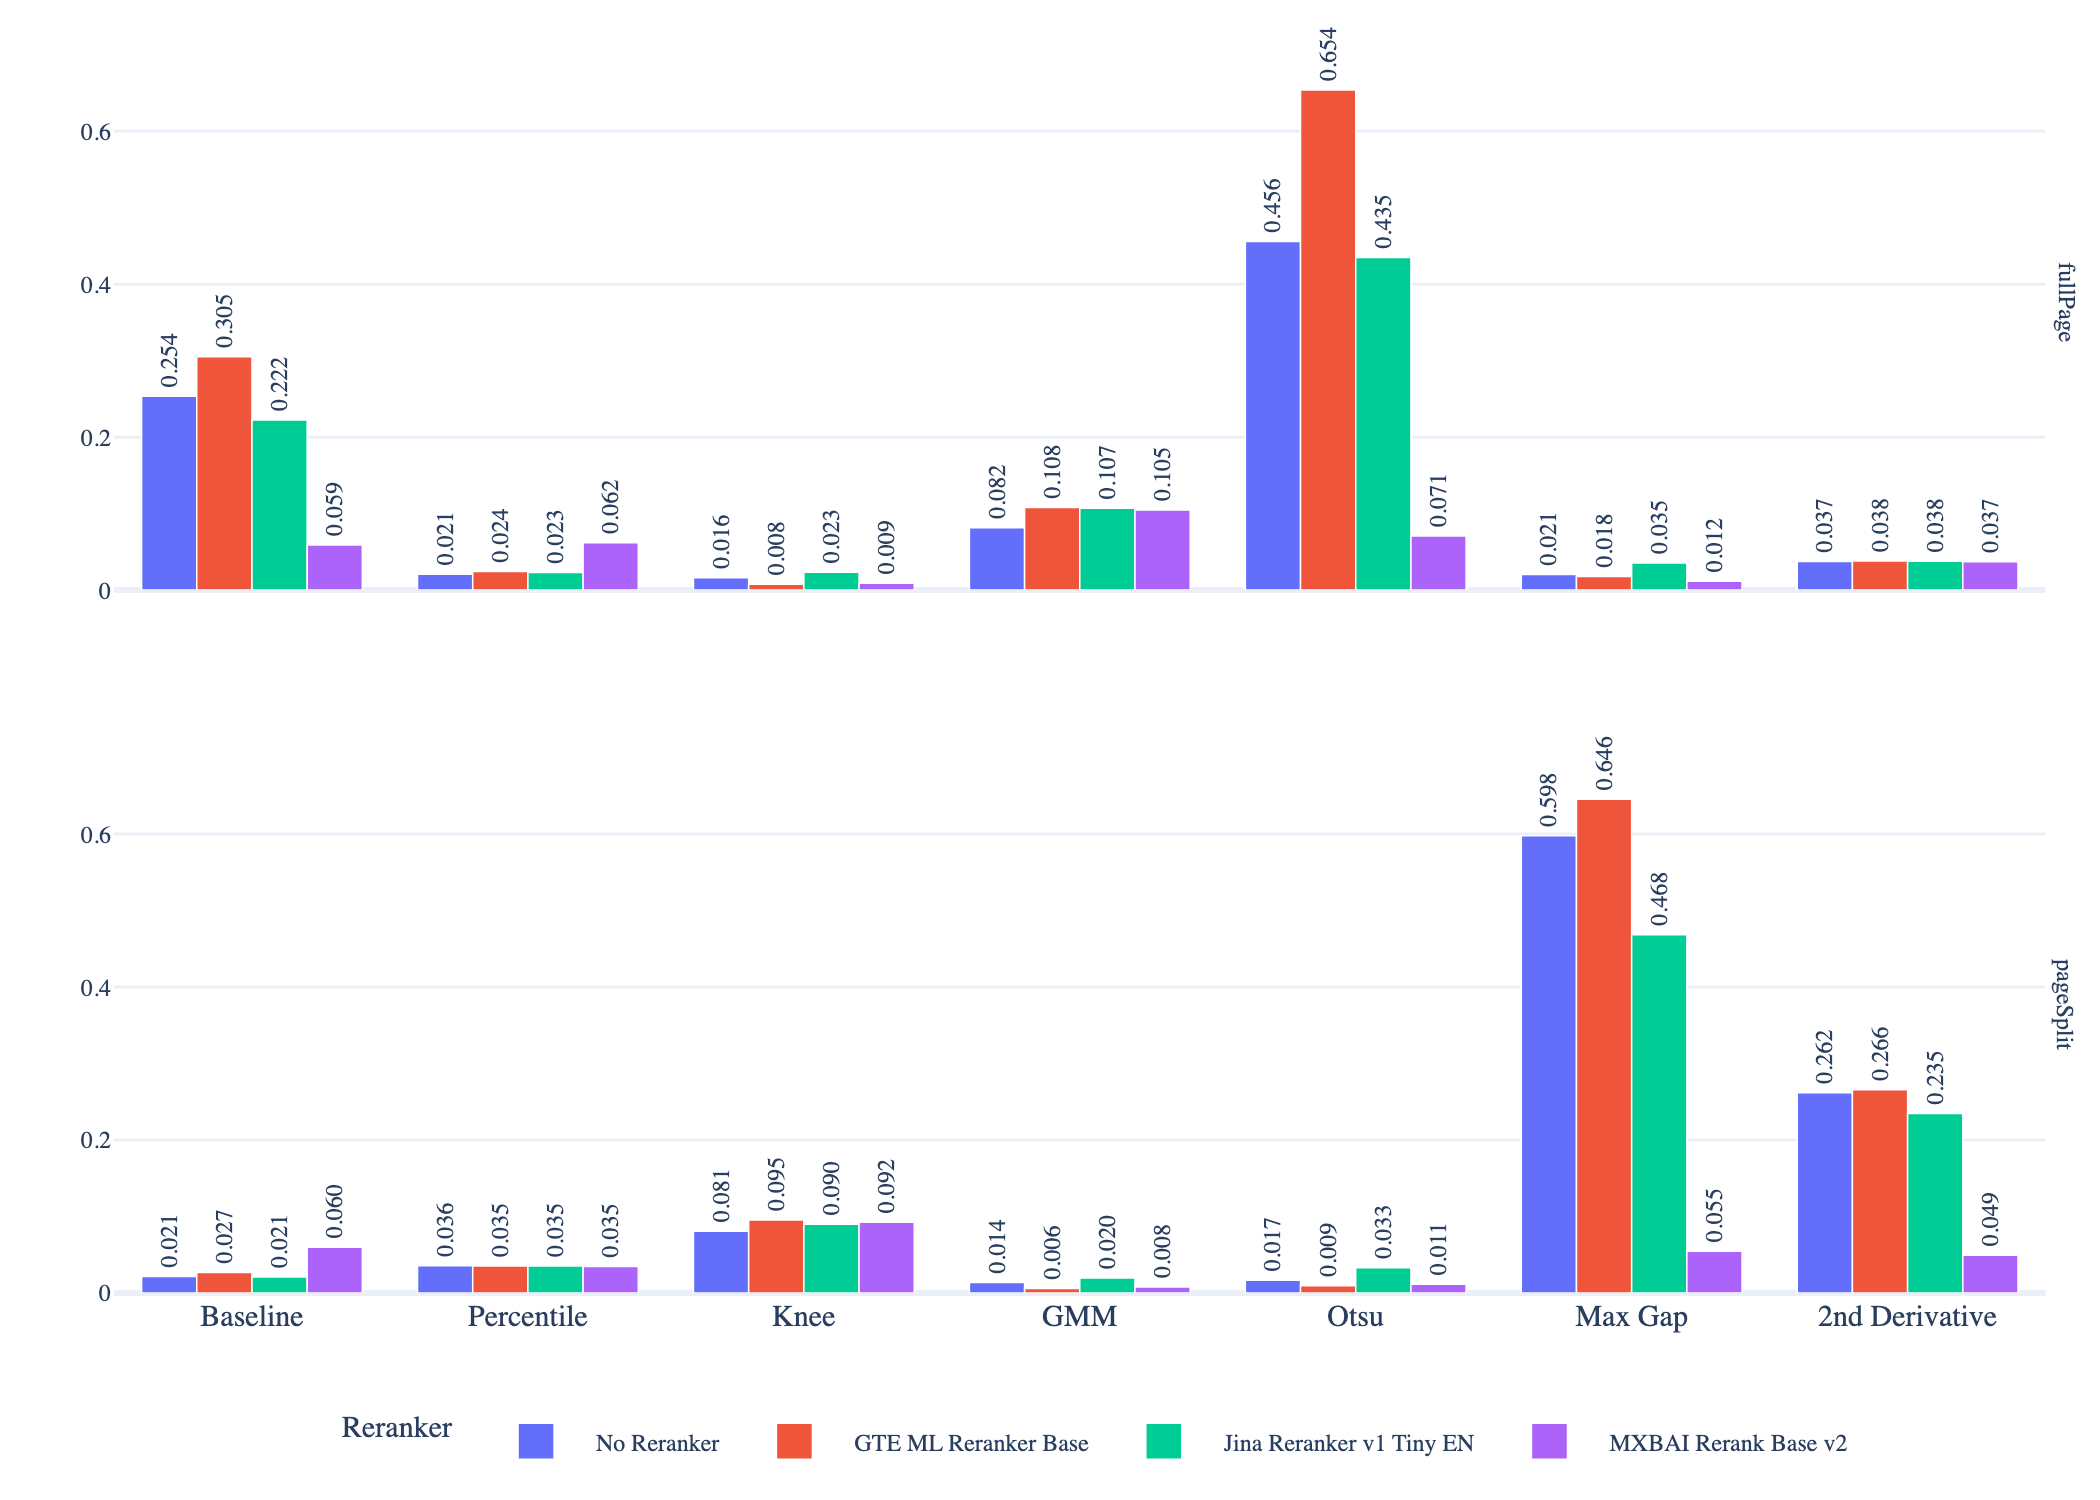
\includegraphics[width=\textwidth]{reranker/avg_f1_score_bar_faceted.png}
        \\[1ex]\footnotesize (a) Average F1 score by facet
      \end{minipage}
      \hfill
      \begin{minipage}[b]{0.49\textwidth}
        \centering
        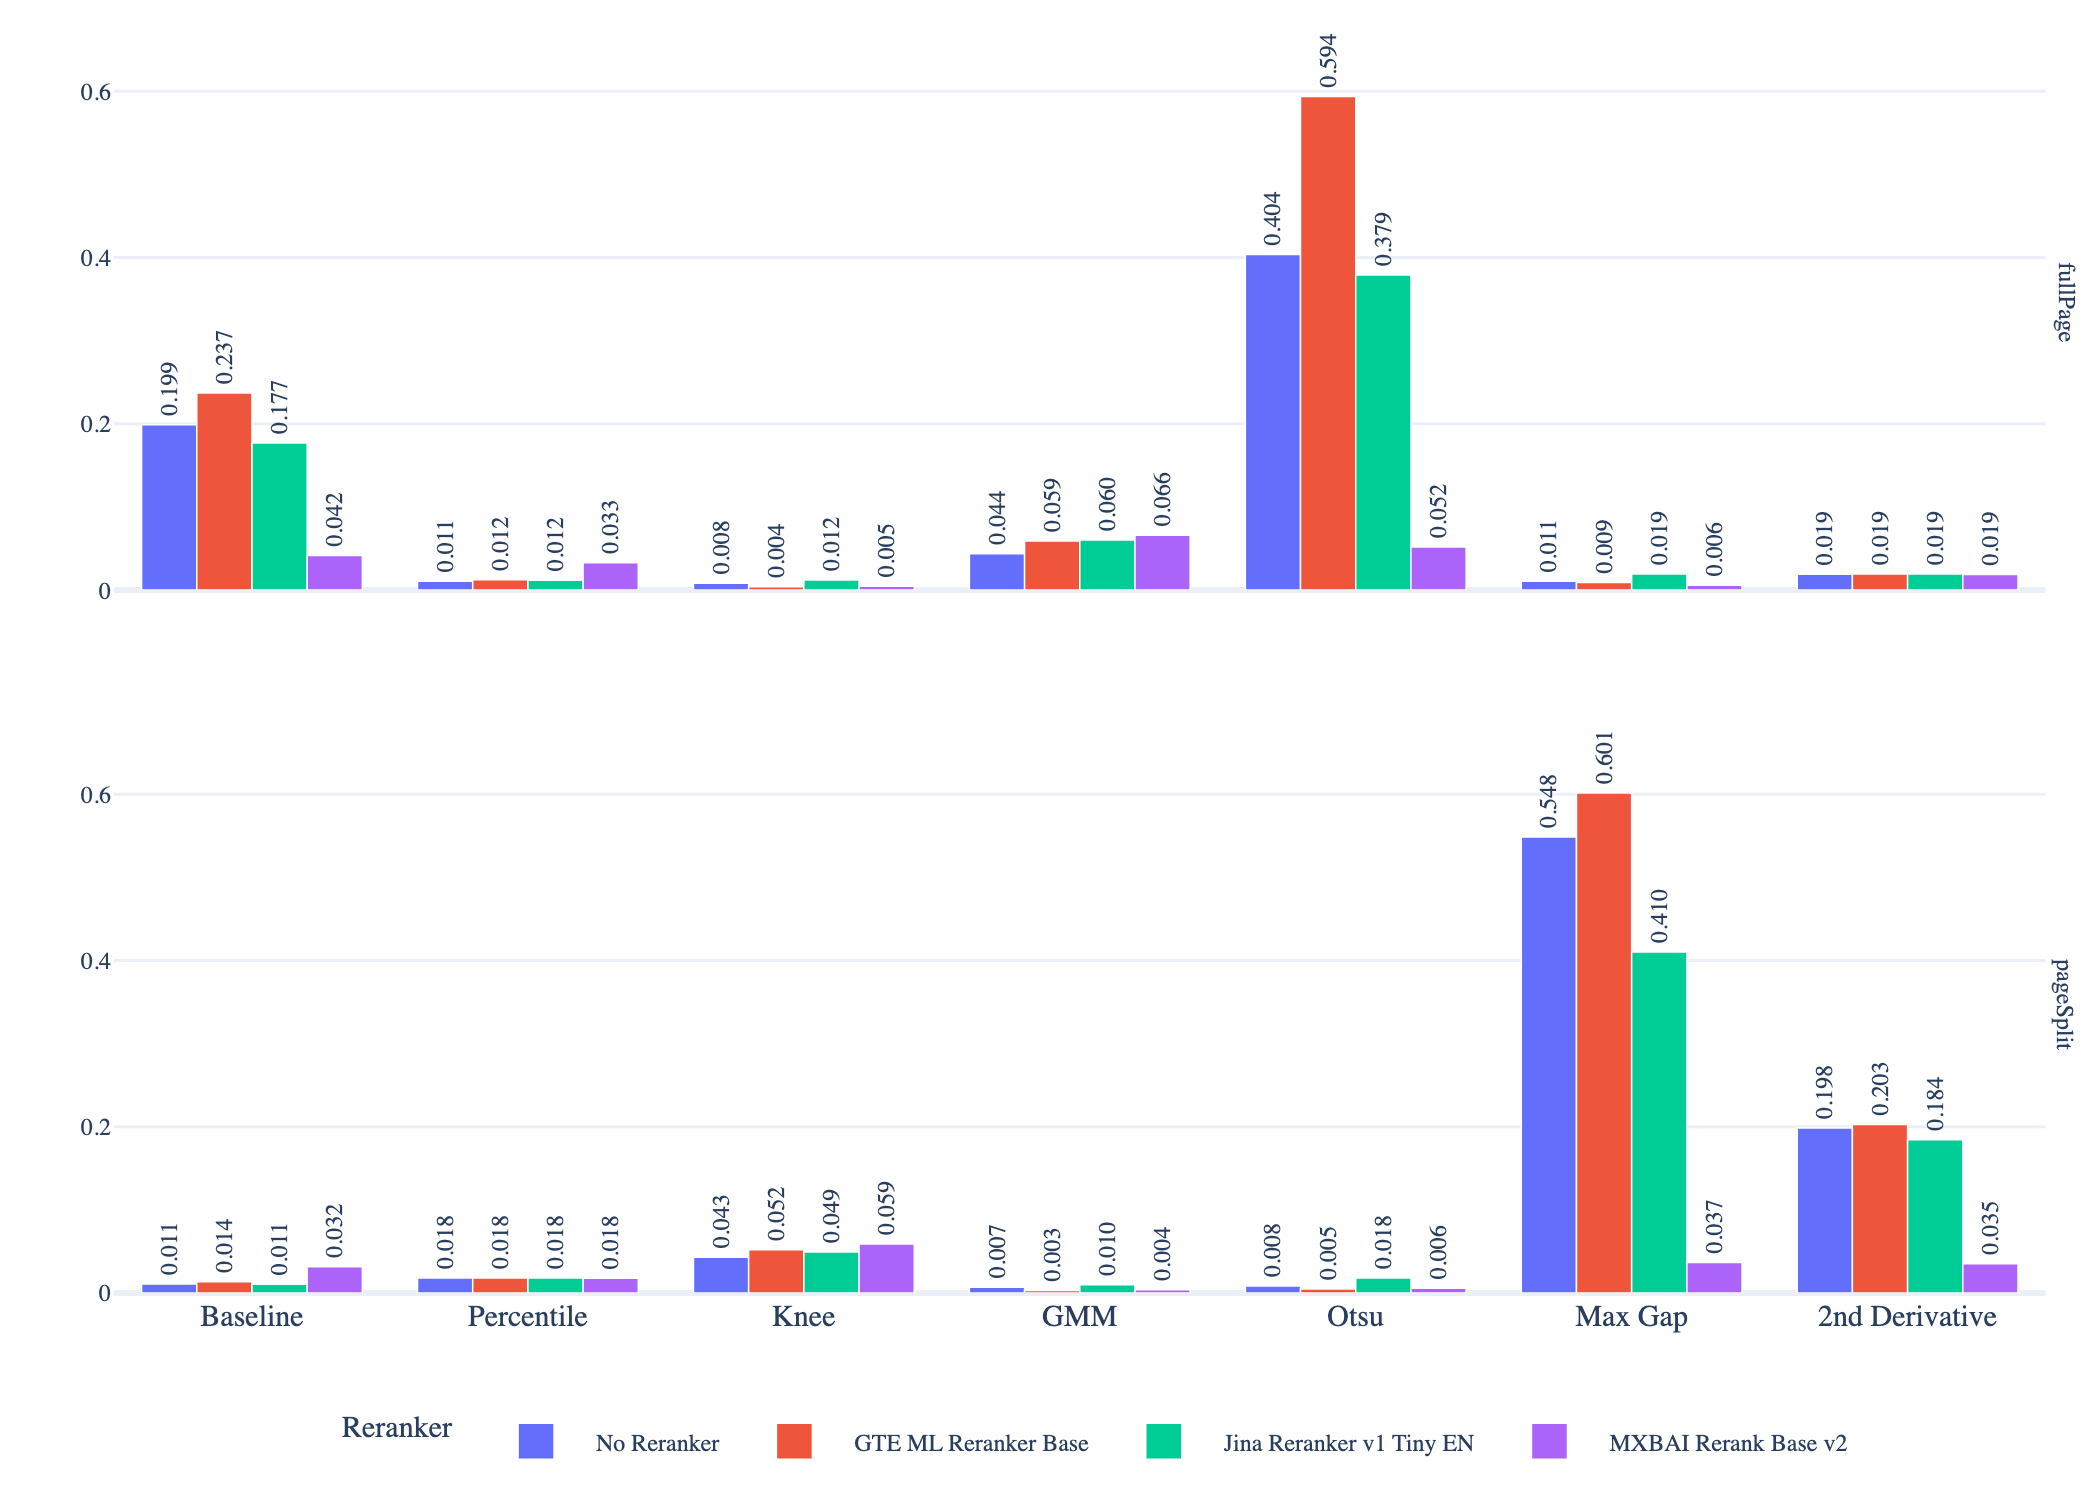
\includegraphics[width=\textwidth]{reranker/avg_precision_bar_faceted.png}
        \\[1ex]\footnotesize (b) Average precision by facet
      \end{minipage}

      \vspace{1ex}

      % second row: recall
      \begin{minipage}[b]{0.49\textwidth}
        \centering
        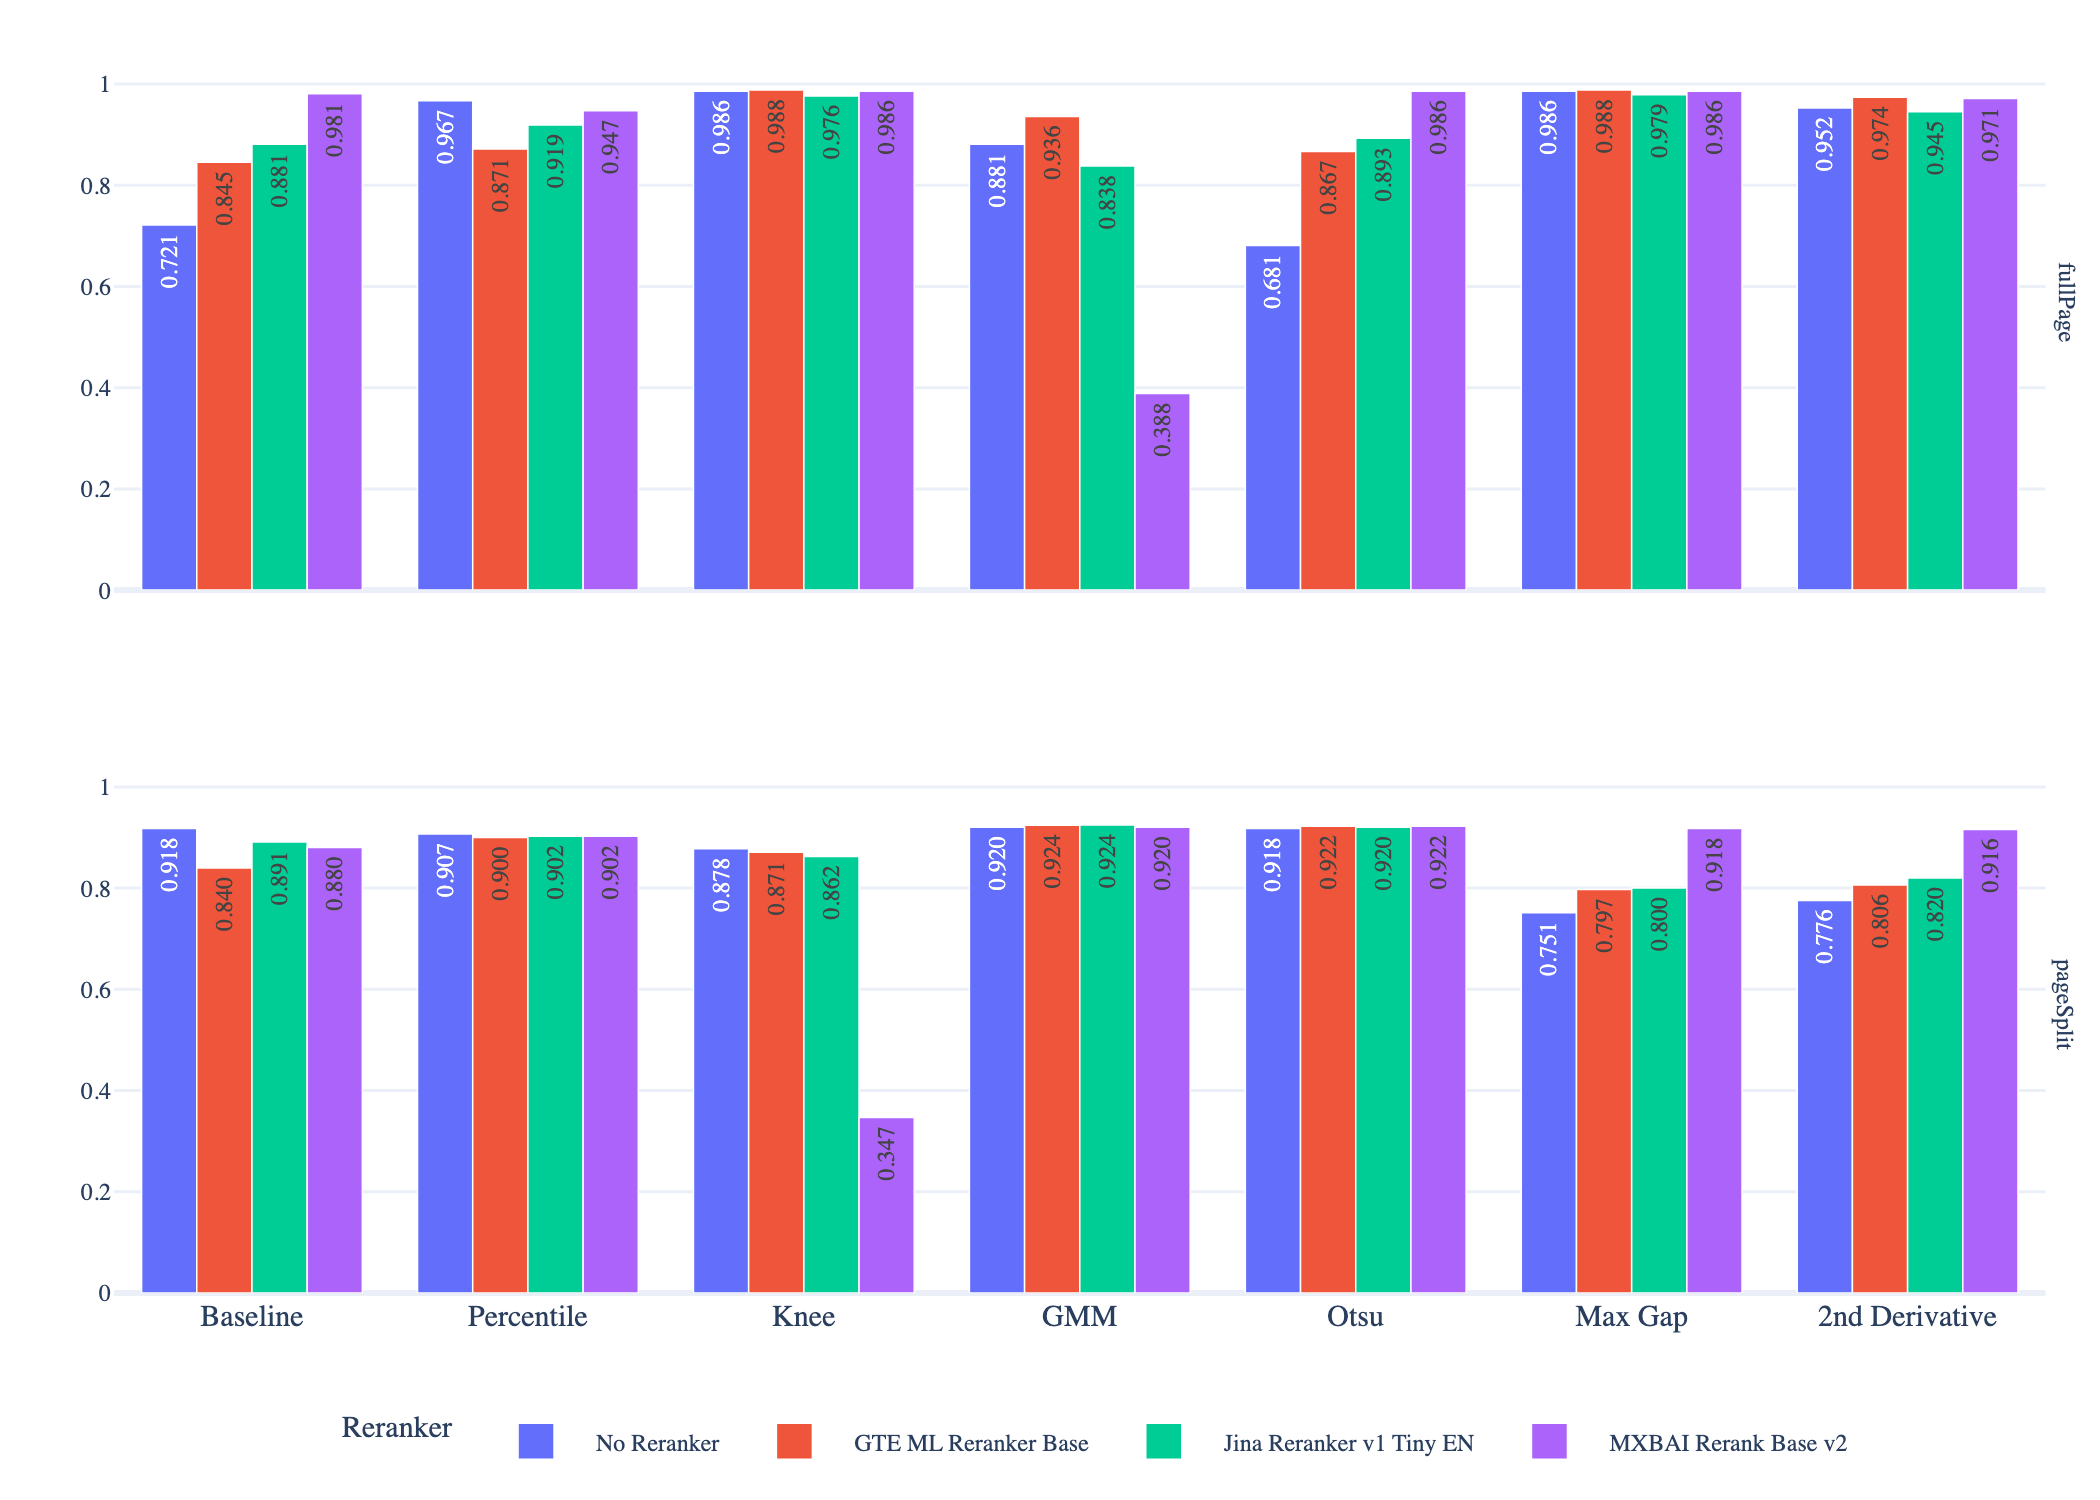
\includegraphics[width=\textwidth]{reranker/avg_recall_bar_faceted.png}
        \\[1ex]\footnotesize (c) Average recall by facet
      \end{minipage}

      \vspace{1ex}

      % third row: items & retrieved docs
      \begin{minipage}[b]{0.49\textwidth}
        \centering
        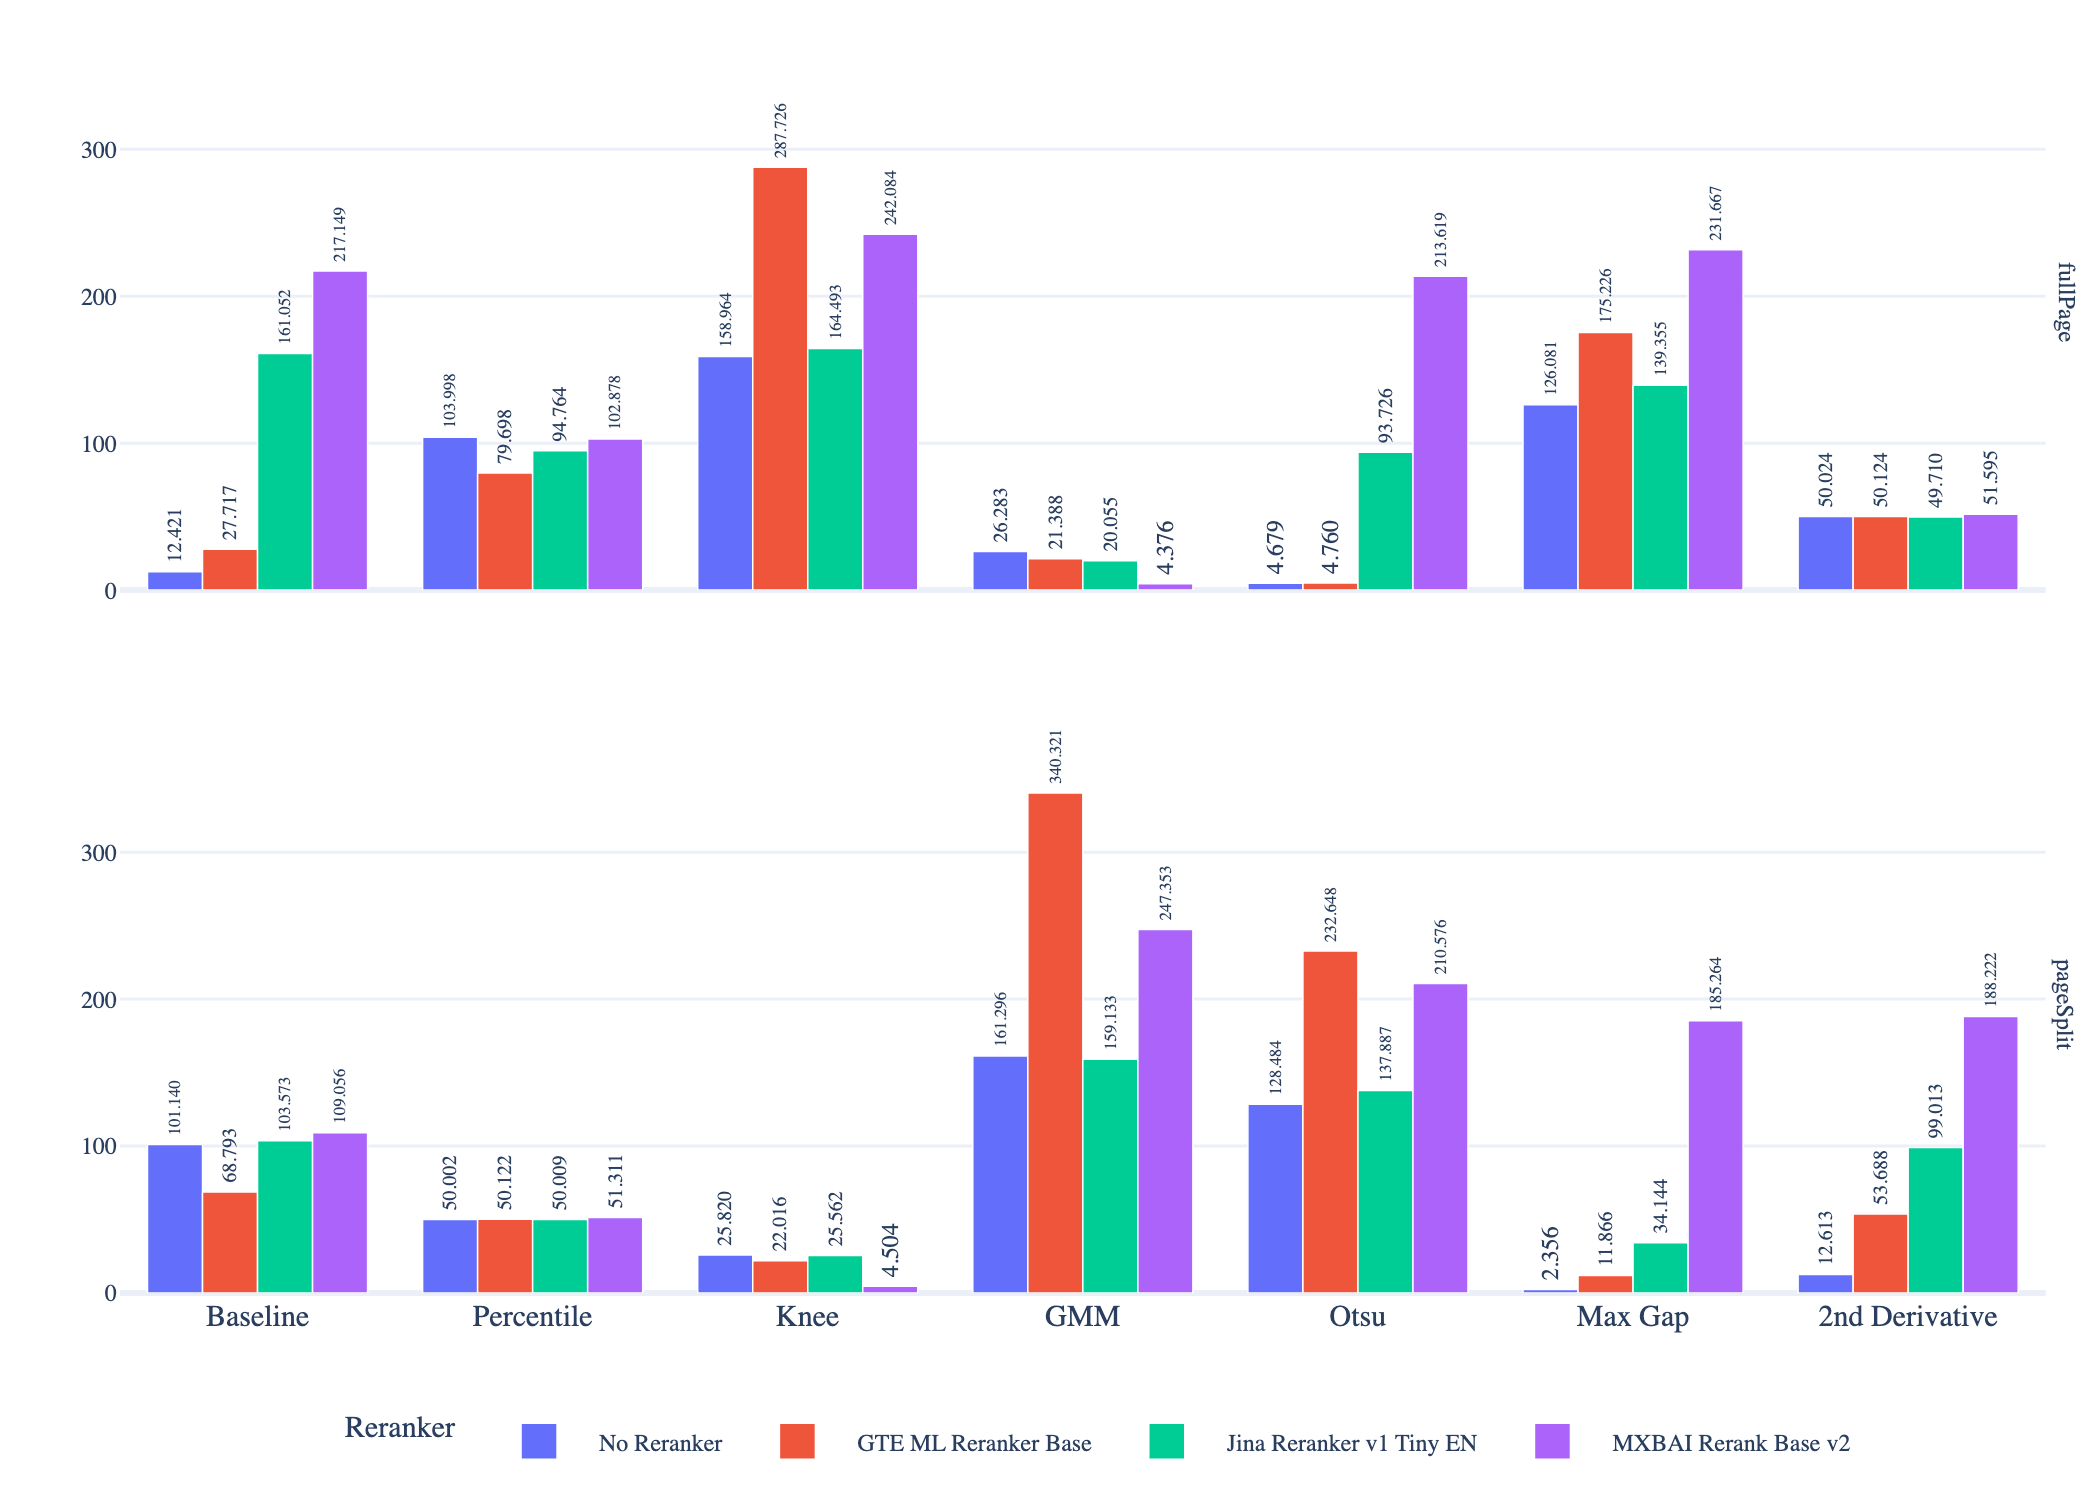
\includegraphics[width=\textwidth]{reranker/avg_num_items_passed_bar_faceted.png}
        \\[1ex]\footnotesize (d) Average number of items passed by facet
      \end{minipage}
      \hfill
      \begin{minipage}[b]{0.49\textwidth}
        \centering
        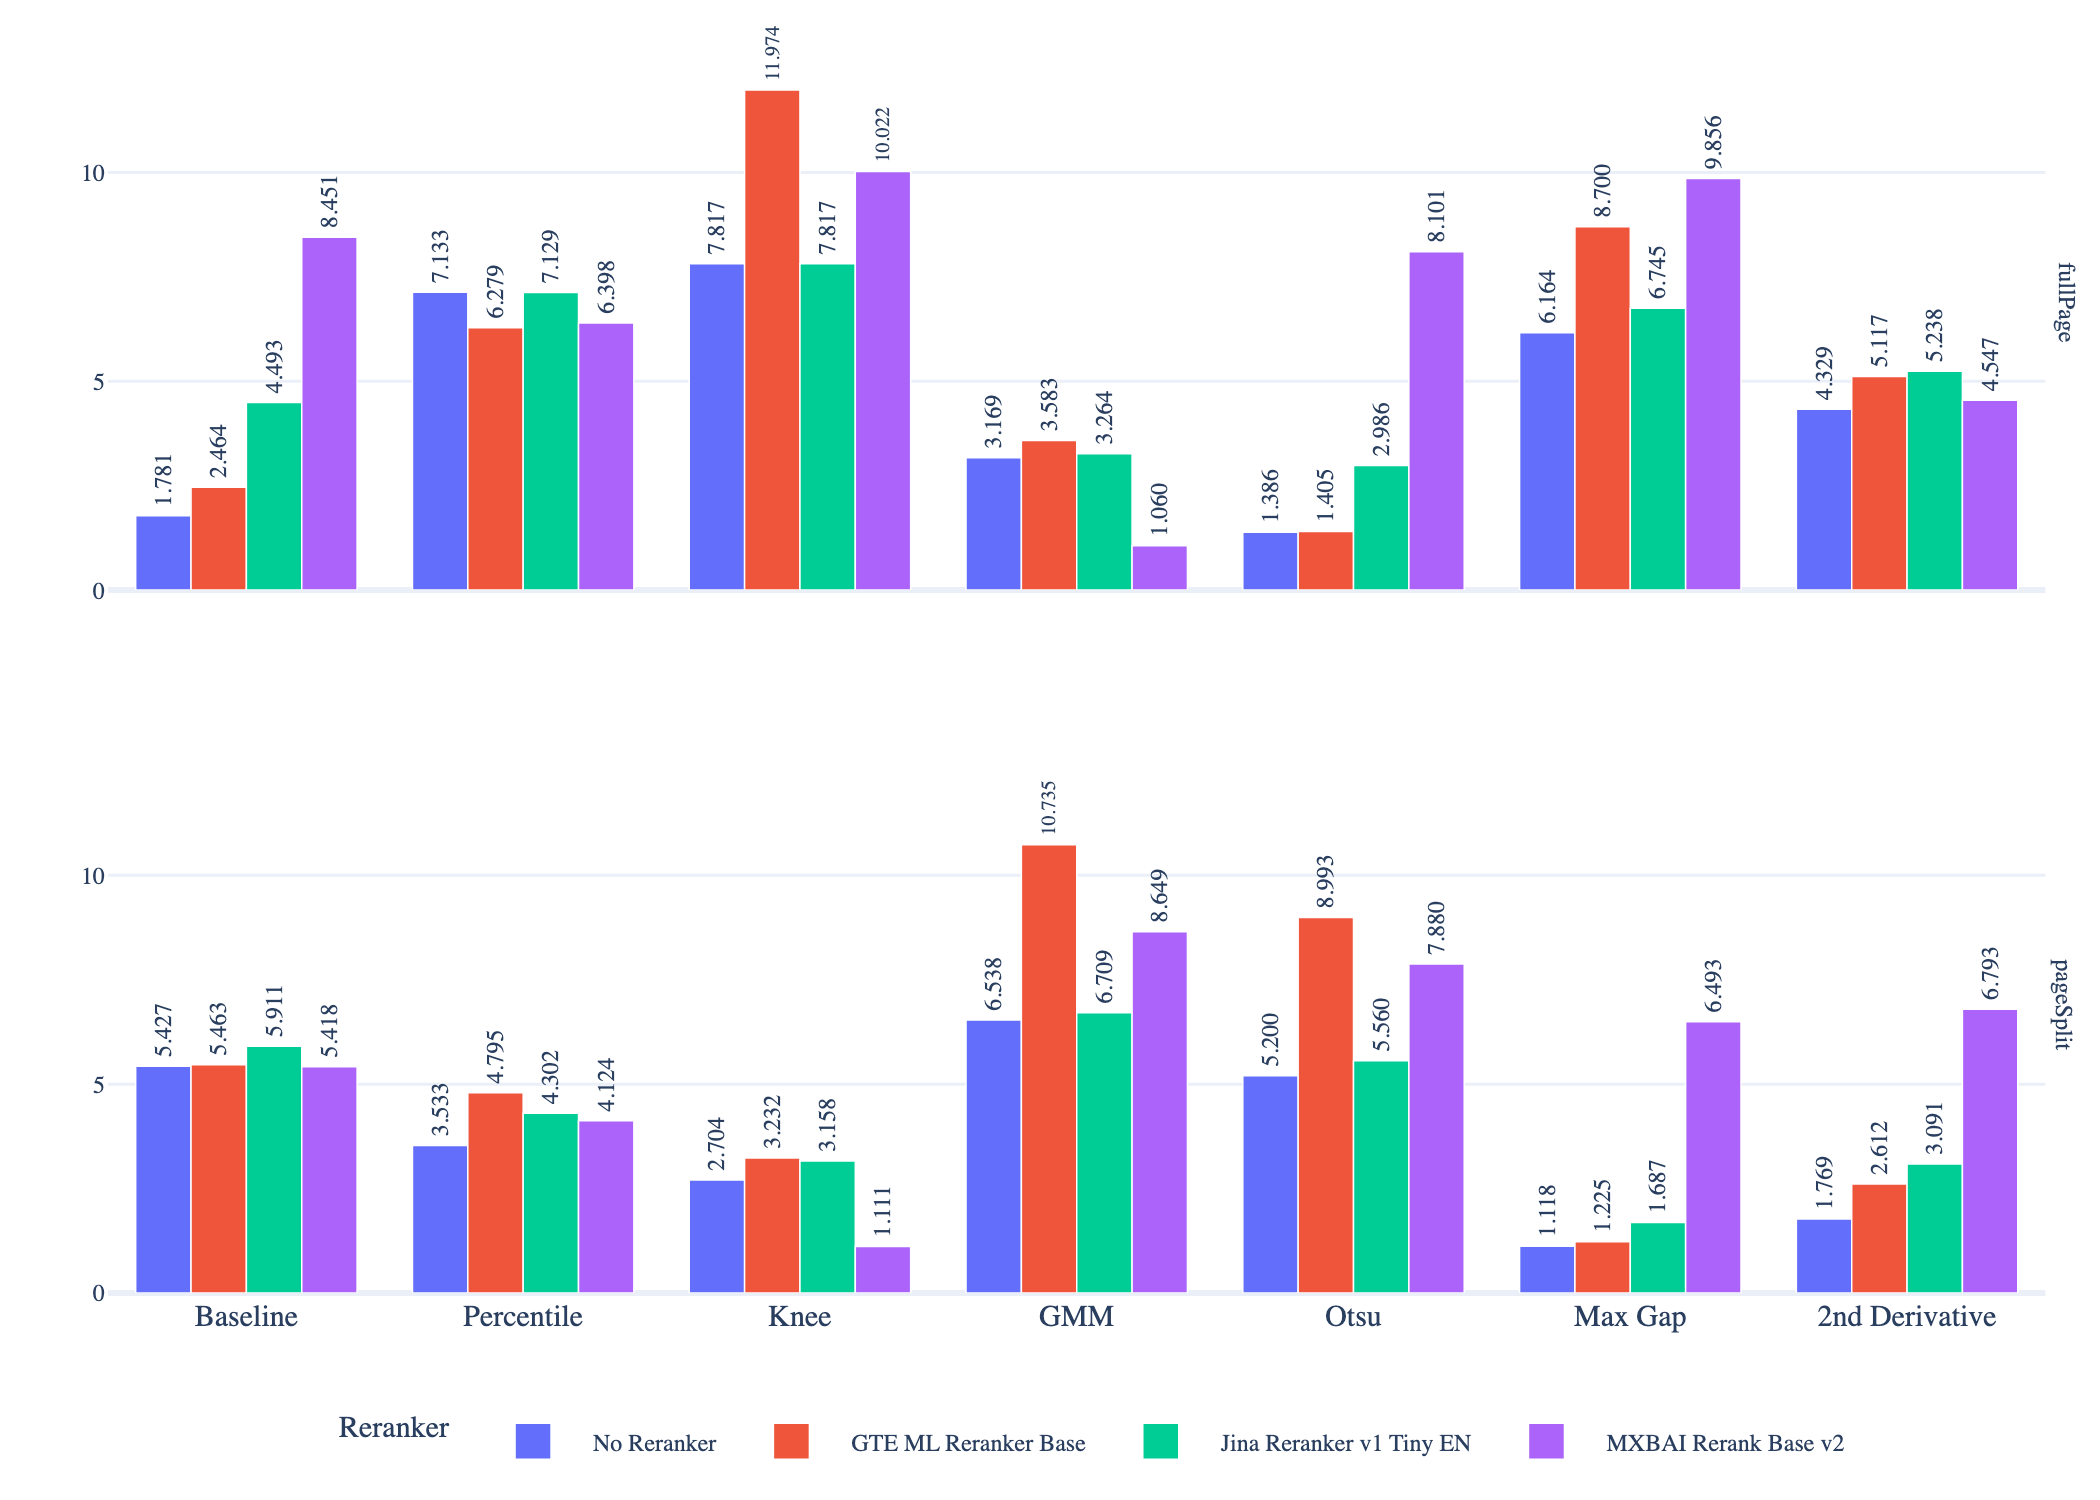
\includegraphics[width=\textwidth]{reranker/avg_num_retrieved_docs_passed_bar_faceted.png}
        \\[1ex]\footnotesize (e) Average number of retrieved documents passed by facet
      \end{minipage}
    \end{minipage}% 
  }
  \caption{\footnotesize Comparison of average metrics by model facet:
    (a) F1 score, (b) precision, (c) recall, (d) number of items passed,
    and (e) number of retrieved documents passed.}
  \label{fig:avg_metrics_faceted}
\end{figure}

\section{Experiment 3: Prompt Engineering to Prevent Hallucination}
\label{sec:exp_generator_prompt}
This experiment centers on the generation component of the RAG pipeline, assessing a broad spectrum of Large Language Models to function as the generator. The primary objective was to identify the optimal-performing model and the most suitable prompt and temperature configuration for our specific use case.

\subsection{Motivation and Baseline}
The evaluation commenced with a baseline configuration of \textbf{GPT-4o} employing prompt \texttt{P1} and a temperature of \texttt{0.2}. As novel and more powerful models were introduced during the course of this research, they were systematically evaluated against this baseline. This continuous evaluation process enabled us to remain at the forefront of research and select the most suitable model for integration into a production RAG system, thereby ensuring that any replacement would provide superior performance.

\subsection{Evaluation Methodology}
We utilized the \textbf{DeepEval} framework \autocite{deepeval2023}, which employs an LLM-as-a-Judge approach to assess the generator's output. For subjective, use-case-specific evaluations, we employed DeepEval's \textbf{G-Eval} functionality, which draws inspiration from the G-Eval framework \autocite{liu2023geval} and utilizes a chain-of-thought process to evaluate outputs against custom criteria. We delineated two such metrics:
\begin{itemize}
    \item \textbf{Correctness (C):} This metric ascertains whether the actual output is factually correct based on the expected output. It heavily penalizes the omission of crucial details and the inclusion of information that contradicts the expected output.
    \item \textbf{Specific Information Accuracy (SIA):} This metric evaluates whether the model's response appropriately utilizes information from the context without introducing specific details (names, places, numbers) that are not explicitly provided. It is particularly important for assessing the model's capacity to discern when a question cannot be answered from the provided context. For example, a high SIA score is conferred if the model accurately indicates its inability to answer a question such as "Who is Cinderella?" when presented with an anonymized version of the story, as this demonstrates its non-reliance on its internal parametric knowledge.
\end{itemize}

In addition to our custom G-Eval metrics, we employed several of DeepEval's standard metrics to assess other critical qualities of the generated output:
\begin{itemize}
    \item \textbf{Answer Relevancy (AR):} This metric quantifies the relevance of the generated output to the user's input query. It ensures that the model's response is pertinent and directly addresses the posed question \autocite{deepeval2023}.
    \item \textbf{Faithfulness (F):} This metric evaluates whether the generated output factually corresponds with the information present in the retrieved context. A high score indicates that the model did not fabricate facts and adhered faithfully to the source material \autocite{deepeval2023}.
    \item \textbf{Hallucination (H):} This metric ascertains if the model generates factually incorrect information by comparing the output to the provided context. It is a critical measure for ensuring the trustworthiness of the RAG system \autocite{deepeval2023}.
\end{itemize}


\subsection{Results and Discussion}
The comprehensive results are delineated in Table \ref{tab:deepeval_results}. The baseline configuration (GPT-4o, P1, Temp 0.2) yielded a total score of 370.52. The results indicate that several newer models and prompt configurations were capable of significantly outperforming this baseline.

For instance, the \textbf{O4 Mini} model employing prompt \texttt{P2} and a temperature of \texttt{0.2} attained the highest total score of \textbf{403.86}. This demonstrates the utility of continuous evaluation, as it enabled us to identify a model that not only performs superiorly to the original baseline but also to ascertain the optimal prompt (\texttt{P2}) and temperature (\texttt{0.2}) for it. These findings are crucial for deploying a RAG system that is not only accurate and faithful but also robust in addressing queries that cannot be answered from the available context.

\begin{landscape}
    \footnotesize
    \setlength{\tabcolsep}{3pt}       % default is ~6pt
    \renewcommand{\arraystretch}{0.9}  % tighten row height
    \setlength{\LTleft}{0pt}          % left align longtable
    \setlength{\LTright}{0pt}         % right align longtable
    \begin{longtable}{|l|c|c|ccccc|c|ccccc|ccccc|}
        \caption{DeepEval Generative Model and Prompt Evaluation Results}
        \label{tab:deepeval_results} \\

        \toprule
        \textbf{Model} & \textbf{Prompt} & \textbf{Temp} & \multicolumn{5}{c|}{\textbf{Avg. Scores}} & \textbf{Total} & \multicolumn{5}{c|}{\textbf{GPT-4o}} & \multicolumn{5}{c|}{\textbf{Claude 3.5}} \\
        & & & \textbf{AR} & \textbf{C} & \textbf{F} & \textbf{H} & \textbf{SIA} & & \textbf{AR} & \textbf{C} & \textbf{F} & \textbf{H} & \textbf{SIA} & \textbf{AR} & \textbf{C} & \textbf{F} & \textbf{H} & \textbf{SIA} \\
        \midrule
        \endfirsthead

        \multicolumn{19}{c}{\tablename\ \thetable{} -- continued from previous page} \\
        \midrule
        \textbf{Model} & \textbf{Prompt} & \textbf{Temp} & \textbf{AR} & \textbf{C} & \textbf{F} & \textbf{H} & \textbf{SIA} & \textbf{Total} & \textbf{AR} & \textbf{C} & \textbf{F} & \textbf{H} & \textbf{SIA} & \textbf{AR} & \textbf{C} & \textbf{F} & \textbf{H} & \textbf{SIA} \\
        \midrule
        \endhead

        \midrule
        \multicolumn{19}{l}{\footnotesize{\textbf{AR}: Answer Relevancy, \textbf{C}: Correctness, \textbf{F}: Faithfulness, \textbf{H}: Hallucination, \textbf{SIA}: Specific Information Accuracy}} \\
        \multicolumn{19}{r}{Continued on next page} \\ 
        \endfoot

        \bottomrule
        \multicolumn{19}{l}{\footnotesize{\textbf{AR}: Answer Relevancy, \textbf{C}: Correctness, \textbf{F}: Faithfulness, \textbf{H}: Hallucination, \textbf{SIA}: Specific Information Accuracy}}
        \endlastfoot
        Claude 3 Haiku & P1 & 0.0 & 57.70 & 66.66 & 87.18 & 69.23 & 74.36 & 355.13 & 61.54 & 69.23 & 84.62 & 64.10 & 79.49 & 53.85 & 64.10 & 89.74 & 74.36 & 69.23 \\
        Claude 3 Haiku & P1 & 0.2 & 62.82 & 61.54 & 87.18 & 65.38 & 67.94 & 344.86 & 61.54 & 53.85 & 84.62 & 58.97 & 64.10 & 64.10 & 69.23 & 89.74 & 71.79 & 71.79 \\
        Claude 3 Haiku & P2 & 0.0 & 66.66 & 62.82 & 89.74 & 67.94 & 74.36 & 361.52 & 64.10 & 56.41 & 89.74 & 64.10 & 82.05 & 69.23 & 69.23 & 89.74 & 71.79 & 66.67 \\
        Claude 3 Haiku & P2 & 0.2 & 62.82 & 61.53 & 79.49 & 65.38 & 73.07 & 342.29 & 61.54 & 58.97 & 79.49 & 58.97 & 82.05 & 64.10 & 64.10 & 79.49 & 71.79 & 64.10 \\
        Claude 3.5 Sonnet & P1 & 0.0 & 58.97 & 76.93 & 92.31 & 74.35 & 71.79 & 374.35 & 61.54 & 69.23 & 97.44 & 58.97 & 71.79 & 56.41 & 84.62 & 87.18 & 89.74 & 71.79 \\
        Claude 3.5 Sonnet v2 & P1 & 0.0 & 48.72 & 75.65 & 96.16 & 66.66 & 67.95 & 355.14 & 48.72 & 66.67 & 92.31 & 51.28 & 69.23 & 48.72 & 84.62 & 100.00 & 82.05 & 66.67 \\
        Claude 3.5 Sonnet v2 & P1 & 0.2 & 52.56 & 69.23 & 96.16 & 71.80 & 69.23 & 358.98 & 53.85 & 53.85 & 94.87 & 56.41 & 76.92 & 51.28 & 84.62 & 97.44 & 87.18 & 61.54 \\
        Claude 3.5 Sonnet v2 & P2 & 0.0 & 62.82 & 70.52 & 91.03 & 78.20 & 84.62 & 387.19 & 64.10 & 61.54 & 89.74 & 61.54 & 84.62 & 61.54 & 79.49 & 92.31 & 94.87 & 84.62 \\
        Claude 3.5 Sonnet v2 & P2 & 0.2 & 64.10 & 75.64 & 94.87 & 76.92 & 88.46 & 399.99 & 71.79 & 74.36 & 94.87 & 61.54 & 89.74 & 56.41 & 76.92 & 94.87 & 92.31 & 87.18 \\
        Claude 3.7 Sonnet & P1 & 0.0 & 48.72 & 82.05 & 88.47 & 71.80 & 78.20 & 369.24 & 48.72 & 69.23 & 92.31 & 56.41 & 74.36 & 48.72 & 94.87 & 84.62 & 87.18 & 82.05 \\
        Claude 3.7 Sonnet & P1 & 0.2 & 44.87 & 88.46 & 88.46 & 73.08 & 88.46 & 383.33 & 46.15 & 87.18 & 94.87 & 58.97 & 94.87 & 43.59 & 89.74 & 82.05 & 87.18 & 82.05 \\
        Claude 3.7 Sonnet & P2 & 0.0 & 48.72 & 78.21 & 93.59 & 78.20 & 85.90 & 384.62 & 53.85 & 71.79 & 94.87 & 61.54 & 79.49 & 43.59 & 84.62 & 92.31 & 94.87 & 92.31 \\
        Claude 3.7 Sonnet & P2 & 0.2 & 43.59 & 84.62 & 89.74 & 79.49 & 92.31 & 389.75 & 46.15 & 82.05 & 89.74 & 66.67 & 92.31 & 41.03 & 87.18 & 89.74 & 92.31 & 92.31 \\
        Claude 4.0 Sonnet & P1 & 0.2 & 38.46 & 83.34 & 89.75 & 76.92 & 83.33 & 371.80 & 38.46 & 79.49 & 87.18 & 61.54 & 89.74 & 38.46 & 87.18 & 92.31 & 92.31 & 76.92 \\
        Claude 4.0 Sonnet & P2 & 0.2 & 42.31 & 84.62 & 91.03 & 79.49 & 91.03 & 388.48 & 41.03 & 84.62 & 97.44 & 66.67 & 94.87 & 43.59 & 84.62 & 84.62 & 92.31 & 87.18 \\
        GPT-4 Omni & P1 & 0.0 & 56.41 & 65.38 & 93.59 & 70.52 & 67.94 & 353.84 & 53.85 & 58.97 & 92.31 & 56.41 & 71.79 & 58.97 & 71.79 & 94.87 & 84.62 & 64.10 \\
        GPT-4 Omni & P1 & 0.2 & 60.26 & 78.20 & 92.31 & 67.95 & 71.80 & 370.52 & 53.85 & 74.36 & 94.87 & 51.28 & 69.23 & 66.67 & 82.05 & 89.74 & 84.62 & 74.36 \\
        GPT-4 Omni & P2 & 0.0 & 56.41 & 74.36 & 92.31 & 61.54 & 78.20 & 362.82 & 51.28 & 64.10 & 92.31 & 48.72 & 76.92 & 61.54 & 84.62 & 92.31 & 74.36 & 79.49 \\
        GPT-4 Omni & P2 & 0.2 & 58.97 & 73.08 & 92.31 & 67.95 & 79.48 & 371.79 & 53.85 & 61.54 & 92.31 & 56.41 & 82.05 & 64.10 & 84.62 & 92.31 & 79.49 & 76.92 \\
        GPT-4 Omni Mini & P1 & 0.0 & 61.54 & 73.08 & 91.03 & 70.52 & 66.66 & 362.83 & 51.28 & 71.79 & 89.74 & 56.41 & 69.23 & 71.79 & 74.36 & 92.31 & 84.62 & 64.10 \\
        GPT-4 Omni Mini & P1 & 0.2 & 61.54 & 71.80 & 94.88 & 69.23 & 70.52 & 367.97 & 56.41 & 69.23 & 92.31 & 53.85 & 74.36 & 66.67 & 74.36 & 97.44 & 84.62 & 66.67 \\
        GPT-4 Omni Mini & P2 & 0.0 & 65.38 & 74.36 & 92.31 & 57.69 & 75.64 & 365.38 & 66.67 & 69.23 & 92.31 & 43.59 & 79.49 & 64.10 & 79.49 & 92.31 & 71.79 & 71.79 \\
        GPT-4 Omni Mini & P2 & 0.2 & 64.10 & 76.92 & 91.03 & 58.97 & 80.77 & 371.79 & 64.10 & 71.79 & 87.18 & 46.15 & 82.05 & 64.10 & 82.05 & 94.87 & 71.79 & 79.49 \\
        GPT-4.1 & P1 & 0.2 & 65.38 & 82.05 & 93.59 & 73.07 & 85.89 & 399.98 & 64.10 & 82.05 & 97.44 & 56.41 & 89.74 & 66.67 & 82.05 & 89.74 & 89.74 & 82.05 \\
        GPT-4.1 & P2 & 0.2 & 62.82 & 80.77 & 93.59 & 70.52 & 89.74 & 397.44 & 61.54 & 76.92 & 94.87 & 61.54 & 89.74 & 64.10 & 84.62 & 92.31 & 79.49 & 89.74 \\
        GPT-4.1 Nano & P1 & 0.2 & 56.41 & 69.23 & 93.59 & 75.64 & 73.08 & 367.95 & 58.97 & 61.54 & 92.31 & 58.97 & 71.79 & 53.85 & 76.92 & 94.87 & 92.31 & 74.36 \\
        GPT-4.1 Nano & P2 & 0.2 & 65.38 & 57.69 & 87.18 & 69.23 & 78.20 & 357.68 & 64.10 & 51.28 & 89.74 & 58.97 & 79.49 & 66.67 & 64.10 & 84.62 & 79.49 & 76.92 \\
        Gemini 1.5 Flash & P1 & 0.0 & 73.08 & 61.53 & 93.59 & 62.82 & 65.39 & 356.41 & 69.23 & 58.97 & 92.31 & 51.28 & 61.54 & 76.92 & 64.10 & 94.87 & 74.36 & 69.23 \\
        Gemini 1.5 Flash & P1 & 0.2 & 73.08 & 57.69 & 96.16 & 61.54 & 67.95 & 356.42 & 71.79 & 51.28 & 94.87 & 48.72 & 69.23 & 74.36 & 64.10 & 97.44 & 74.36 & 66.67 \\
        Gemini 1.5 Flash & P2 & 0.0 & 78.20 & 52.56 & 96.16 & 69.23 & 67.95 & 364.10 & 76.92 & 51.28 & 97.44 & 53.85 & 66.67 & 79.49 & 53.85 & 94.87 & 84.62 & 69.23 \\
        Gemini 1.5 Flash & P2 & 0.2 & 78.20 & 67.95 & 92.31 & 69.23 & 82.06 & 389.75 & 82.05 & 66.67 & 92.31 & 53.85 & 79.49 & 74.36 & 69.23 & 92.31 & 84.62 & 84.62 \\
        Gemini 1.5 Pro & P1 & 0.0 & 74.36 & 60.26 & 93.59 & 65.39 & 56.41 & 350.01 & 74.36 & 53.85 & 100.00 & 43.59 & 53.85 & 74.36 & 66.67 & 87.18 & 87.18 & 58.97 \\
        Gemini 1.5 Pro & P1 & 0.2 & 75.64 & 52.56 & 91.03 & 64.11 & 55.13 & 338.47 & 74.36 & 48.72 & 94.87 & 43.59 & 56.41 & 76.92 & 56.41 & 87.18 & 84.62 & 53.85 \\
        Gemini 1.5 Pro & P2 & 0.0 & 67.94 & 56.41 & 97.44 & 65.38 & 65.38 & 352.55 & 64.10 & 51.28 & 97.44 & 51.28 & 71.79 & 71.79 & 61.54 & 97.44 & 79.49 & 58.97 \\
        Gemini 1.5 Pro & P2 & 0.2 & 74.36 & 58.97 & 93.59 & 60.25 & 74.36 & 361.53 & 71.79 & 58.97 & 92.31 & 46.15 & 74.36 & 76.92 & 58.97 & 94.87 & 74.36 & 74.36 \\
        Gemini 2.0 Flash & P1 & 0.0 & 48.72 & 48.72 & 97.44 & 65.39 & 53.84 & 314.11 & 51.28 & 46.15 & 97.44 & 43.59 & 48.72 & 46.15 & 51.28 & 97.44 & 87.18 & 58.97 \\
        Gemini 2.0 Flash & P1 & 0.2 & 47.44 & 46.16 & 100.00 & 58.98 & 56.41 & 308.99 & 46.15 & 41.03 & 100.00 & 33.33 & 48.72 & 48.72 & 51.28 & 100.00 & 84.62 & 64.10 \\
        Gemini 2.0 Flash & P2 & 0.0 & 66.66 & 61.53 & 93.59 & 67.95 & 74.36 & 364.09 & 64.10 & 58.97 & 92.31 & 56.41 & 71.79 & 69.23 & 64.10 & 94.87 & 79.49 & 76.92 \\
        Gemini 2.0 Flash & P2 & 0.2 & 73.08 & 56.41 & 92.31 & 65.38 & 75.64 & 362.82 & 71.79 & 51.28 & 92.31 & 51.28 & 74.36 & 74.36 & 61.54 & 92.31 & 79.49 & 76.92 \\
        Gemini 2.5 Flash & P2 & 0.2 & 55.12 & 74.36 & 91.03 & 69.23 & 85.90 & 375.64 & 51.28 & 66.67 & 92.31 & 56.41 & 87.18 & 58.97 & 82.05 & 89.74 & 82.05 & 84.62 \\
        Gemini 2.5 Flash & P2 & 0.2 & 57.70 & 75.64 & 91.03 & 74.35 & 87.18 & 385.90 & 53.85 & 74.36 & 94.87 & 58.97 & 89.74 & 61.54 & 76.92 & 87.18 & 89.74 & 84.62 \\
        Gemini 2.5 Flash & P2 & 0.2 & 62.82 & 78.20 & 91.03 & 70.52 & 87.18 & 389.75 & 58.97 & 76.92 & 92.31 & 56.41 & 89.74 & 66.67 & 79.49 & 89.74 & 84.62 & 84.62 \\
        Gemini 2.5 Flash & P2 & 0.2 & 66.66 & 74.36 & 89.75 & 69.23 & 88.46 & 388.46 & 58.97 & 66.67 & 92.31 & 53.85 & 87.18 & 74.36 & 82.05 & 87.18 & 84.62 & 89.74 \\
        Gemini 2.5 Pro & P2 & 0.2 & 62.82 & 82.05 & 93.59 & 73.08 & 91.03 & 402.57 & 61.54 & 74.36 & 94.87 & 61.54 & 94.87 & 64.10 & 89.74 & 92.31 & 84.62 & 87.18 \\
        Gemini 2.5 Pro & P2 & 0.2 & 62.82 & 82.05 & 89.74 & 71.80 & 88.46 & 394.87 & 66.67 & 71.79 & 89.74 & 58.97 & 89.74 & 58.97 & 92.31 & 89.74 & 84.62 & 87.18 \\
        Gemini 2.5 Pro & P2 & 0.2 & 57.69 & 76.93 & 92.31 & 75.64 & 87.18 & 389.75 & 58.97 & 69.23 & 97.44 & 61.54 & 87.18 & 56.41 & 84.62 & 87.18 & 89.74 & 87.18 \\
        Gemini 2.5 Pro & P2 & 0.2 & 62.82 & 78.21 & 88.47 & 76.92 & 87.18 & 393.60 & 58.97 & 69.23 & 92.31 & 64.10 & 89.74 & 66.67 & 87.18 & 84.62 & 89.74 & 84.62 \\
        O1 & P1 & 0.0 & 66.67 & 82.05 & 93.59 & 76.92 & 84.62 & 403.85 & 71.79 & 76.92 & 94.87 & 56.41 & 87.18 & 61.54 & 87.18 & 92.31 & 97.44 & 82.05 \\
        O1 & P2 & 0.0 & 70.52 & 71.79 & 97.44 & 62.82 & 93.59 & 396.16 & 66.67 & 64.10 & 97.44 & 46.15 & 92.31 & 74.36 & 79.49 & 97.44 & 79.49 & 94.87 \\
        O3 & P1 & 0.2 & 75.64 & 66.67 & 88.47 & 69.23 & 78.20 & 378.21 & 76.92 & 74.36 & 61.54 & 71.79 & 84.62 & 92.31 & 53.85 & 84.62 & 76.92 & 79.49 \\
        O3 & P2 & 0.2 & 70.51 & 80.77 & 91.03 & 73.07 & 85.89 & 401.27 & 71.79 & 71.79 & 89.74 & 56.41 & 82.05 & 69.23 & 89.74 & 92.31 & 89.74 & 89.74 \\
        O3 Mini & P1 & 0.0 & 70.52 & 67.95 & 96.16 & 74.36 & 62.82 & 371.81 & 74.36 & 56.41 & 94.87 & 61.54 & 66.67 & 66.67 & 79.49 & 97.44 & 87.18 & 58.97 \\
        O3 Mini & P1 & 0.2 & 60.25 & 65.38 & 93.59 & 67.95 & 65.39 & 352.56 & 64.10 & 48.72 & 94.87 & 51.28 & 61.54 & 56.41 & 82.05 & 92.31 & 84.62 & 69.23 \\
        O3 Mini & P2 & 0.0 & 64.11 & 74.36 & 92.31 & 74.36 & 75.64 & 380.78 & 61.54 & 69.23 & 89.74 & 66.67 & 74.36 & 66.67 & 79.49 & 94.87 & 82.05 & 76.92 \\
        O3 Mini & P2 & 0.2 & 65.38 & 71.80 & 96.16 & 69.23 & 79.49 & 382.06 & 66.67 & 61.54 & 94.87 & 56.41 & 79.49 & 64.10 & 82.05 & 97.44 & 82.05 & 79.49 \\
        O4 Mini & P1 & 0.2 & 67.95 & 75.64 & 93.59 & 73.07 & 83.34 & 393.59 & 69.23 & 66.67 & 76.92 & 74.36 & 94.87 & 92.31 & 56.41 & 89.74 & 84.62 & 82.05 \\
        O4 Mini & P2 & 0.2 & 74.36 & 83.34 & 93.59 & 66.67 & 85.90 & 403.86 & 71.79 & 79.49 & 92.31 & 48.72 & 87.18 & 76.92 & 87.18 & 94.87 & 84.62 & 84.62 \\
    \end{longtable}
\end{landscape}

\subsection{Comparative Analysis Against GPT-4o}
\label{sec:comparative_analysis_gpt4o}

To better understand the relative performance of each model, we calculated the delta between each model's total score and the baseline score of GPT-4o (370.52). The results are summarized in Table \ref{tab:deepeval_delta_results}.

\begin{table}[!htbp]
\centering
\small
\caption{Total Score Delta vs. GPT-4o (Highest Scores)}
\label{tab:deepeval_delta_results}
\begin{tabular}{|l|c|c|c|}
\hline
\textbf{Model} & \textbf{Prompt} & \textbf{Temp} & \textbf{Delta from GPT-4o} \\
\hline
O4 Mini & P2 & 0.2 & +33.34 \\
O1 & P1 & 0.0 & +33.33 \\
Gemini 2.5 Pro & P2 & 0.2 & +32.05 \\
O3 & P2 & 0.2 & +30.75 \\
Claude 3.5 Sonnet v2 & P2 & 0.2 & +29.47 \\
GPT-4.1 & P1 & 0.2 & +29.46 \\
Claude 3.7 Sonnet & P2 & 0.2 & +19.23 \\
Gemini 1.5 Flash & P2 & 0.2 & +19.23 \\
Gemini 2.5 Flash & P2 & 0.2 & +19.23 \\
Claude 4.0 Sonnet & P2 & 0.2 & +17.96 \\
O3 Mini & P2 & 0.2 & +11.54 \\
Claude 3.5 Sonnet & P1 & 0.0 & +3.83 \\
GPT-4 Omni Mini & P2 & 0.2 & +1.27 \\
GPT-4 Omni & P2 & 0.2 & +1.27 \\
\hline
\multicolumn{4}{|c|}{\textbf{GPT-4o Baseline Total Score: 370.52}} \\
\hline
GPT-4.1 Nano & P1 & 0.2 & -2.57 \\
Gemini 2.0 Flash & P2 & 0.0 & -6.43 \\
Claude 3 Haiku & P2 & 0.0 & -9.00 \\
Gemini 1.5 Pro & P2 & 0.2 & -9.00 \\
\hline
\end{tabular}
\end{table}

\subsubsection{Inference from the Results}
The delta analysis reveals several key insights. Firstly, the top-performing models, such as \textbf{O4 Mini}, \textbf{O1}, and \textbf{Gemini 2.5 Pro}, show a significant improvement over the GPT-4o baseline, with score increases exceeding 30 points. This underscores the rapid advancements in generative models, where newer architectures can yield substantial performance gains.

Secondly, the choice of prompt and temperature settings is evidently crucial. For many models, there is a considerable performance variance between different prompt versions (P1 vs. P2) and temperature settings. For instance, the O1 model with prompt P1 scores much higher than with P2 (403.85 vs 396.16: +7.69 points). This highlights the necessity of meticulous prompt engineering and parameter tuning to unlock a model's full potential.
